% -*- coding: UTF-8 -*-
% hello.tex

\documentclass[UTF8,oneside]{ctexbook}

% \usepackage{xeCJK}
\usepackage[utf8]{inputenc}

% load paralist before enumitem
\usepackage{paralist}

\usepackage{hyperref}
\hypersetup{pdftex,colorlinks=true,allcolors=blue}
\usepackage{hypcap}

\usepackage{color}
\usepackage[usenames, dvipsnames, svgnames, table]{xcolor}
% \pagecolor{gray}

\usepackage{makeidx}
\makeindex

\usepackage{amsmath}
\usepackage{mathtools}

\usepackage{listings}
\usepackage{multicol}
\usepackage{fancybox}
\usepackage{tcolorbox}
\usepackage{enumitem}

\usepackage{indentfirst}

\newenvironment{enumbox}[0]{
    \begin{tcolorbox}
    \begin{compactenum}
} {
    \end{compactenum}
    \end{tcolorbox}
}

\newenvironment{itembox}[0]{
    \begin{tcolorbox}
    \begin{compactitem}
} {
    \end{compactitem}
    \end{tcolorbox}
}

% table
\setlength{\arrayrulewidth}{1pt}
\setlength{\tabcolsep}{16pt}
\renewcommand{\arraystretch}{2.5}
\newcolumntype{s}{>{\columncolor[HTML]{AAACED}} p{3cm}}

\arrayrulecolor[HTML]{DB5800}

\usepackage{tikz,mathpazo}
\usetikzlibrary{positioning, fit, matrix, shapes, arrows, chains, trees, arrows.meta}

% \bibliographystyle{plain}
% \bibliography{math}

\tikzset{%
  >={Latex[width=2mm,length=2mm]},
  % Specifications for style of nodes:
            base/.style = {rectangle, rounded corners, draw=black,
                           minimum width=4cm, minimum height=1cm,
                           text centered, font=\sffamily},
  activityStarts/.style = {base, fill=blue!30},
       startstop/.style = {base, fill=red!30},
    activityRuns/.style = {base, fill=green!30},
         process/.style = {base, minimum width=2.5cm, fill=orange!15,
                           font=\ttfamily},
}

% 摘录
\usepackage{verbatim}
\usepackage{libertine}
\usepackage{graphicx}
\usepackage{framed}

\newcommand*\openquote{\makebox(25,-22){\scalebox{5}{``}}}
\newcommand*\closequote{\makebox(25,-22){\scalebox{5}{''}}}
\colorlet{shadecolor}{Azure}

\makeatletter
\newif\if@right
\def\shadequote{\@righttrue\shadequote@i}
\def\shadequote@i{\begin{snugshade}\begin{quote}\openquote}
\def\endshadequote{%
\if@right\hfill\fi\closequote\end{quote}\end{snugshade}}
\@namedef{shadequote*}{\@rightfalse\shadequote@i}
\@namedef{endshadequote*}{\endshadequote}
\makeatother

\usepackage[normalem]{ulem}

\newcommand{\hl}{\bgroup\markoverwith
  {\textcolor{yellow}{\rule[-.5ex]{2pt}{2.5ex}}}\ULon}

%\usepackage{soul}

%\newcommand{\hlc}[2][yellow]{{%
%    \colorlet{foo}{#1}%
%    \sethlcolor{foo}\hl{#2}}%
%}

% todonode
\usepackage{lipsum}                     % Dummytext
\usepackage{xargs}                      % Use more than one optional parameter in a new commands
% 
\usepackage[colorinlistoftodos,prependcaption,textsize=tiny]{todonotes}
\newcommandx{\unsure}[2][1=]{\todo[linecolor=red,backgroundcolor=red!25,bordercolor=red,#1]{#2}}
\newcommandx{\change}[2][1=]{\todo[linecolor=blue,backgroundcolor=blue!25,bordercolor=blue,#1]{#2}}
\newcommandx{\info}[2][1=]{\todo[linecolor=OliveGreen,backgroundcolor=OliveGreen!25,bordercolor=OliveGreen,#1]{#2}}
\newcommandx{\improvement}[2][1=]{\todo[linecolor=Plum,backgroundcolor=Plum!25,bordercolor=Plum,#1]{#2}}
\newcommandx{\thiswillnotshow}[2][1=]{\todo[disable,#1]{#2}}
%

\usepackage[simplified]{pgf-umlcd}

\title{LICH架构文档}
\author{董冠军}
\date{\today}

\begin{document}

\maketitle
\tableofcontents

\listoftodos[Notes]

\part{项目管理}

\chapter{移动集采}

产品评估:功能和质量。质量包括:可靠性,性能,QoS,可扩展性(负载均衡),用户体验(管控,交互,接口)等方面。

性能不是一个值,而是不同场景下的特征曲线。性能是系统配置和负载的函数:$P=F(S, W)$。
精简配置,快照,故障,实现机制等因素都会影响性能及其抖动。

\section{CheckList}

对标\hl{移动集采测试规范}

\subsection{Hardware}

同质化项:
\begin{enumbox}
\item 开机Logo
\item 贴标
\item 开机卡,需断电源
\end{enumbox}

\subsection{Software}

标前测试:
\begin{enumbox}
\item 管理系统相关Logo
\item 上架
\item 安装
\item 性能测试
\end{enumbox}

BUG
\begin{enumbox}
\item etcd依赖于物理时间
\item bcache拔cache盘后需要重启服务器
\end{enumbox}

性能:
\begin{enumbox}
\item \hl{打开chunk parallel开关}
\item \hl{禁用core}
\item 优化Log
\item O3编译
\item -g
\item 代码段
\end{enumbox}

功能:
\begin{enumbox}
\item IPv6
\item SNMP
\item bcache
\item Recovery
\item Balance
\item QoS
\item QoS 1.1抖动幅度是否需要可配置
\end{enumbox}

\section{LEFT}

\subsection{可靠性}

诊断写错误效率太低,需要完善分析方法和工具。

log分析法

chunk,副本级数据一致性校验(disk bitmap和sqlite)。

disk bitmap无,而sqlite有。会导致什么结果?多个sqlite记录指向同一个磁盘位置。

\subsection{性能}

clock(副本一致性)

msqqueue(操作日志)

卷分为chunk,chunk有多副本。在独立的部分之间,尽量并发。

多个卷,要注意session和controller平衡。

在分配阶段,一个chunk的持久化信息,包括三部分:diskmd,sqlite和table2 meta。

并发,锁的粒度。

\subsection{删除}

删除卷,比删除快照更早完成,导致快照无法删除

回收replica时,sqlite有,disk bitmap无。

并发删除一个卷的多个快照会如何?

有节点不在线,无法完成删卷操作,反复重试而无果。

timer不工作,是堵塞还是其它?

删除队列里的快照,也计入快照数,满足一下不等式:root+auto+rmsnap+user <= 256。

提供强制回收的工具

\subsection{平衡}

批量分配卷

\subsection{md5sum}

每个chunk有几种状态:没分配,分配,分配并填0。
第一种和第三种状态等价,第二种状态结果不可知。

\section{TODO}

\begin{enumbox}
\item Pool
\item Volume size
\item Volume mv and copy
\item Volume IOPS QOS
\item Mapping
%\item Recovery
%\item 可靠性 Robustness
%\item Load Balance
%\item Performance
\item extentability
\end{enumbox}

\section{重要问题}

\subsection{存储池}

模型:概念及其关系。

重建状态和速度按存储池进行统计。

\subsection{卷}

\begin{enumbox}
\item 精简配置
\item 三副本
\item 扩容
\item 卷的QoS:IOPS
\item 全量拷贝和增量拷贝
\end{enumbox}

三副本 \info{三副本性能}

\subsection{快照}

\begin{enumbox}
\item 显示卷和快照的创建时间,名称,宿主,\hl{容量,存储池}。
\item 快照树是必须的
\item 快照验证:每个快照关联一个数据集。
\end{enumbox}

\subsection{映射}

数据访问和隔离机制,应按\hl{最小权限原则设计}。主机仅能访问映射到该主机的卷

\subsection{故障处理}

\begin{enumbox}
\item IO抖动
\item 重建
\end{enumbox}

\subsection{数据恢复}

触发策略,QoS,性能,状态。

\begin{enumbox}
\item 在线调整策略:应用优先,或恢复优先。
\item 负载调整到原来的20\%时,数据重建效率。
\item 显示恢复速度和状态,区分实际重构的,和跳过的
\item 拔出硬盘的存储池降级(数据冗余度发生下降,目前恢复进程是节点级的,与存储池没有直接关系,并且,在节点的维度上,存储池是有覆盖的,overlay network,\hl{按卷进行汇总})
\item 磁盘漫游,存储系统不发生重建,且数据无异常
\item 模拟故障:单磁盘,单节点,单机架。要求:无读写中断。
\end{enumbox}

要研究的问题:
\begin{enumbox}
\item 在业务负载限定为标准负载的20\%的情况下,恢复性能如何?
\item 如业务IO和数据恢复并存,数据恢复会挤压到很小。原因是什么?\hl{如何做到恢复优先}?
\item 拔盘后,感知状态变化较慢。如\verb|md_chunk_set|不持久化meta,有无副作用?恢复时,也可不持久化。
\end{enumbox}

\subsection{负载均衡}

均衡有数据均衡和负载均衡之分。

单卷的负载均衡,因为FusionStor卷控制器绑定到core上,只能利用单核能力。
CPU利用率上有瓶颈。同时,开启polling模式,会独占core cpu。

\subsection{QoS算法}

卷的IOPS和带宽,数据恢复的QoS,采用同一算法:令牌桶Token bucket。

按恒定速度往桶里加入令牌,任务会消费令牌。如果令牌不足,则任务进入等待状态。
目前,等待时间采用polling策略。等待一个较小的值(200us),唤醒后重新检查。

接口保持不变。

\begin{tcolorbox}
fio队列深度过大,iscsi会有优化,进行IO聚合提交。这样一来,前端工具看到的IOPS可能会有所不同。
但是,各层观察到的带宽应该一致,保证流量守恒。
\end{tcolorbox}

\subsection{Cache}

BCache

\subsection{Misc}

VAAI

\section{不需要做的项}

\begin{enumbox}
\item 一致性组
\item 同步/异步远程复制
\item EC
\end{enumbox}

\chapter{任务清单}

%\pagestyle{empty}
\todo[inline]{The original todo note withouth changed colours.\newline Here's another line.}
\lipsum[11]\unsure{Is this correct?}\unsure{I'm unsure about also!}
\lipsum[11]\change{Change this!}
\lipsum[11]\info{This can help me in chapter seven!}
\lipsum[11]\improvement{This really needs to be improved!\newline\newline What was I thinking?!}
\lipsum[11]
\thiswillnotshow{This is hidden since option `disable' is chosen!}
\improvement[inline]{The following section needs to be rewritten!}
\lipsum[11]
%\newpage

\section{原生卷}

\begin{tcolorbox}
\begin{compactenum}
    \item 存储池
    \item 数据恢复性能
    \item \sout{async sqlite}
    \item \hlc{batch sqlite}
    \item Allocate的性能
    \item 精简配置,快照对性能的影响
    \item 快照树
    \item 单卷快照的数量
    \item SSD Cache
    \item Redis Cache
    \item 异步远程复制
    \item VAAI
    \item FC (+VAAI)
\end{compactenum}
\end{tcolorbox}

\section{关键特性和过程}

\begin{compactenum}
    \item flush, load and recovery
    \item 保护模式 safe mode
    \item 存储分层
    \item 命令行工具,扩展卷和快照相关操作到LSV
\end{compactenum}

\section{兼容性}

\begin{compactenum}
    \item 版本演进
\end{compactenum}

\section{Pool}

\begin{compactenum}
    \item Resource Pool
\end{compactenum}

\section{Volume}

\begin{compactenum}
    \item new format: row2
    \item new format: lsv
    \item vol max size 256T+
    \item vol resize?
    \item all zero's chunk
\end{compactenum}

\section{快照}

\begin{compactenum}
    \item 支持60000+快照
    \item consistency group
    \item 每个snap的大小等信息
    \item snap大小对GC策略的影响
\end{compactenum}

\section{一致性/正确性}

\begin{tcolorbox}
\begin{compactenum}
    \item 底层数据检验工具(chunk0, volume, log/gc, bitmap, wal, rcache)
    \item 内置质量,各模块添加自校验机制,方便诊断数据正确性问题(assert + log + test)
    \item 加强断言:pre和post条件,变量变化规则,不变式,基本假设等
    \item 日志用tag/keywork和timeline,以便于跟踪一个对象的变化历史,用一个或多个维度贯穿起来,用于辅助诊断
    \item 增加CHUNK\_HISTORY,以时间线方式,跟踪记录CHUNK变化的生命周期
\end{compactenum}
\end{tcolorbox}

\section{性能}

性能是负载和资源的函数, $P=F(W, R)$。

\begin{tcolorbox}
\begin{compactenum}
    \item 创建卷时,rcache分配了4096M的SSD cache,可以延迟分配
    \item \textcolor{red}{rcache 顺序IO随机化问题}
    \item wbuf 顺序IO随机化问题
    \item 系统启动时间
    \item 预填充lich chunk
    \item GC策略和算法
    \item 统计基础操作的开销,作为性能分析的基础
\end{compactenum}
\end{tcolorbox}

\section{负载}

\begin{tcolorbox}
\begin{compactenum}
    \item IO队列深度
    \item IO平均大小
    \item IO读写大小
\end{compactenum}
\end{tcolorbox}

\section{资源}

\begin{tcolorbox}
\begin{compactitem}
    \item 内存使用量过大
    \item 内存泄漏
    \item 磁盘利用率不足
    \item 网络带宽:瓶颈或利用率不足
    \item 中断
    \item soft lock up?
\end{compactitem}
\end{tcolorbox}

\section{故障处理}

\begin{compactenum}
    \item \change{故障域,不能中断IO}
    \item 节点间负载均衡(<20\%)
\end{compactenum}

\section{Misc}

\begin{tcolorbox}
\begin{compactitem}
    \item FC
    \item Remote copy
    \item SSD cache
    \item EC
    \item 有效容量的比例
    \item 热插拔
    \item 磁盘漫游
    \item 在线扩容
    \item 滚动升级
\end{compactitem}
\end{tcolorbox}

\section{DONE}

\begin{compactenum}
    \item VAAI [+xcopy]
\end{compactenum}

\chapter{问题集}

\section{空间分配和元数据管理}

目前的空间分配和元数据管理,在支持关键特性和过程上,不够高效。

sqlite层采用(chkid, parent, diskid, offset)指定chkid到磁盘空间的映射。
chkid包含了卷ID,可以利用该信息加快卷的回收过程,但不方便reuse该数据空间。

目前的元数据管理分两层:chunk和replica。
分配一个chunk需要多次IO:
\begin{compactenum}
\item disk bitmap
\item sqlite
\item table2/table1 meta
\end{compactenum}

discard操作与allocate操作顺序相反。

关键过程:
\begin{compactenum}
\item chunk allocate
\item chunk discard (+ reuse)
\end{compactenum}

特性:
\begin{compactenum}
\item replication
\item EC
\end{compactenum}

快照实现:
\begin{compactenum}
\item COW
\item ROW2
\item LSV
\end{compactenum}


\part{测试}

\chapter{测试}

\lstset{numbers=left,
    frame=shadowbox,
    numberstyle= \tiny,
    keywordstyle= \color{ blue!70},commentstyle=\color{red!50!green!50!blue!50}, 
    rulesepcolor= \color{ red!20!green!20!blue!20} 
}

\section{已知问题}

\begin{enumbox}
\item vol resize会产生死锁
\item vol copy的提示
\item flat后保护快照
\end{enumbox}

\section{部署}

基本步骤:
\begin{enumbox}
\item 创建集群
\item 创建存储池
\item 向存储池添加磁盘(Tier, SSD Cache)
\item 创建卷
\item 创建快照
\end{enumbox}

\subsection{创建集群}

\begin{lstlisting}[language=bash]
lich prep t151 t152 t153
lich create t151 t152 t153
\end{lstlisting}

\hl{注意事项}:
\begin{compactenum}
\item 检查IP是否重复
\item 检查子网mask是否匹配
\item ...
\end{compactenum}

\subsection{创建存储池}

\begin{lstlisting}[language=bash]
lichbd pool create p1
\end{lstlisting}

\subsection{向存储池添加磁盘}

\begin{lstlisting}[language=bash]
lich.node --disk_add all --force --pool p1
\end{lstlisting}

\hl{注意事项}:
\begin{compactenum}
\item 存储池内每个节点上需要有SSD,支持tier功能
\item 存储池内每个节点上需要有SSD,支持SSD cache功能
\end{compactenum}

\subsection{创建卷}

\begin{lstlisting}[language=bash]
# 卷路径规范:<pool>/<protocol>/<volume>
# 三副本
# row2格式
lichbd vol create p1/iscsi/v1 --size 4096Gi --repnum 3 -F row2
lich.inspect --localize /iscsi/v1 0 --pool p1
\end{lstlisting}

\hl{注意事项}:
\begin{compactenum}
\item 卷格式:row2 or raw (default)
\item 三副本 (default: 2)
\item 关闭localize
\end{compactenum}

\subsection{创建快照}

\begin{lstlisting}[language=bash]
# 快照路径规范:<pool>/<protocol>/<volume>@<snap>
lichbd snap create p1/iscsi/v1@snap1
\end{lstlisting}

\section{工具}

省略...

\begin{lstlisting}[language=bash]
iscsiadm -m discovery -t st -p 192.168.251.202
\end{lstlisting}

\section{故障测试}

每类节点故障行为不同。除选举过程外,还有vip,iscsi连接,controller的切换,lease,io,恢复过程等。
评价可靠性的指标,主要是vdbench测试中,各种故障条件下io无中断。

另外,故障点还会破坏事务执行的原子性,如allocte过程,创建snapshot过程,
导致严重后果,如造成垃圾,数据状态不一致。如何通过可重入性,或事务解决此类问题?

快照的rollback,delete,flat都设计为可重入过程。如果任务执行失败,可以重新调度。
各种持久化状态之间,保持一致性。

\subsection{单磁盘故障}

磁盘有两种角色:数据盘和cache盘。拔cache盘等同于节点故障?

\subsection{节点故障}

节点有多种角色:
\begin{compactenum}
\item etcd master
\item lich admin
\item lich normal
\end{compactenum}

受VIP机制影响,arp协议会影响客户端到iscsi target的网络连接。
需要注意的是,大部分网络会禁用arp广播,单播则可以。

控制器的加载,lease获取等需要一定时间。


\part{FusionStor}

\chapter{Deploy}

\section{nohosts}

\begin{lstlisting}[frame=single]
[root@node76 ~]# cat /etc/hosts
192.168.1.76 node76
192.168.1.77 node77
192.168.1.78 node78
192.168.1.83 node83

[root@node76 ~]# cat /opt/fusionstack/etc/hosts.conf 
#hosts list for nohost mode
192.168.110.76 node76
192.168.110.77 node77
192.168.110.78 node78
192.168.110.83 node83
\end{lstlisting}

\section{Network}

网段和netmask一致,vip一致

ip addr检查相同IP

arping检查IP冲突 

\section{Disk}

Disk Cache和raid cache下,磁盘读写的行为分析。

如果raid cache打开,writeback写,全随机,则r_await远远大于w_await。
同时,写入的情况下,iostat util较低。



\chapter{硬件架构}

\section{节点}

\subsection{添加节点}

负载均衡,需要重新平衡数据

\subsection{删除节点}

恢复


\section{Pool}

\section{Disk}

\subsection{Tool}

操作磁盘的工具
\begin{enumbox}
\item hdparm set/get hard disk parameters
\item iostat
\item lsscsi
\item udevadm
\item sg\_inq
\item disk2lid
\end{enumbox}

\subsection{Cache}

Disk Cache

关闭磁盘cache,防止出现数据不一致情况。怎么关闭呢?相关管理工具是什么?

磁盘的设备驱动,linux kernel的块设备IO架构

NVMe具有什么特征?

\subsection{RAID}

Ctrl+R进入bios的RAID控制界面。通过bios进行的管理操作,进入系统后用MegaCli等命令行工具也能完成。
且更为方便。

每个控制器管理一个或多个enclosure,每个enclosure有固定数量的slot。每个slot对应一块物理设备。
每个物理设备处在不同的firm 状态,这些状态可以相互转换。在物理设备之上,构建虚拟设备。

带电池BBU的情况下,可以打开RAID cache。

NVMe在不在RAID里,系统盘呢?看不到系统盘,是因为系统盘不在RAID控制器管理的slot内?

缓存盘做出JBOD,数据盘RAID0

全部是JBOD,性能影响较大。

\subsection{Tier}

检测磁盘分层,支持两个磁盘分层:0和1, 0是SSD,1是HDD。

\subsection{Meta}

磁盘管理元数据目录:/opt/fusionstack/data/disk:
\begin{compactitem}
\item disk
\item \hl{bitmap}
\item info
\item tier
\end{compactitem}

对每块磁盘,开头的1M是引导信息,通过bitmap来进行空间管理。
引导信息包含了所在节点信息,所以只能在节点内进行磁盘漫游。

所在源文件是\emph{diskmd.c}。调用fnotify\_register监控磁盘目录的变化,进而添加或移除相应磁盘。

每个节点最多可以添加256个磁盘。

sqlite3划分为10个db文件,chkid信息hash到相应的db。每个db包含两个table:metadata和raw。

\begin{lstlisting}[frame=single]
CREATE TABLE metadata (key text primary key, 
    disk integer, 
    offset integer, 
    parent text, 
    priority integer, 
    meta_version integer, 
    fingerprint integer, 
    wbdisk integer);

CREATE TABLE raw (key text primary key, 
    disk integer, 
    offset integer, 
    parent text, 
    priority integer, 
    meta_version integer, 
    fingerprint integer, 
    wbdisk integer);
\end{lstlisting}

\subsection{状态机}

拔盘-恢复未完成,如何加入?(符号链接丢失,别的文件处在可用状态,重启lichd,修复符号链接)

拔盘-恢复完成,如何加入?

\section{Advanced}

NVMe

RDMA/DPDK/SPDK

AFA

\chapter{架构}

\section{RAID分析}

RAID分析作为架构驱动力

假设和信念
\begin{enumbox}
\item 云是新常态
\item 数据资产是战略资源
\item 全闪是大势所趋
\end{enumbox}

新设计解决了什么老问题?
\begin{enumbox}
\item 单卷的水平扩展问题
\item IO path上的数据转发问题
\item allocate性能低,影响精简配置和COW性能
\item 每个节点导出core、disk等资源,进行全局调度(均衡)
\item 灵活的MM
\item thread local影响CPU利用率
\item ***
\item 重新调整数据布局
\item 单卷大小的限制(支持大卷)
\item chkinfo是动态大小的,副本数、EC配置
\item 底层chunk对象依然不是跨卷的
\item ***
\item COW: volume和snapshot共享对象
\item ***
\item table1/table2实现过于复杂的问题
\item disk md and slots
\item coroutine难于调试
\item ***
\item 多网络
\item MULTIPATH
\item IPv6
\end{enumbox}

\section{模块}

分布式系统架构通常包括几个部分:client、mds、cds。分别对应什么?
\begin{center}
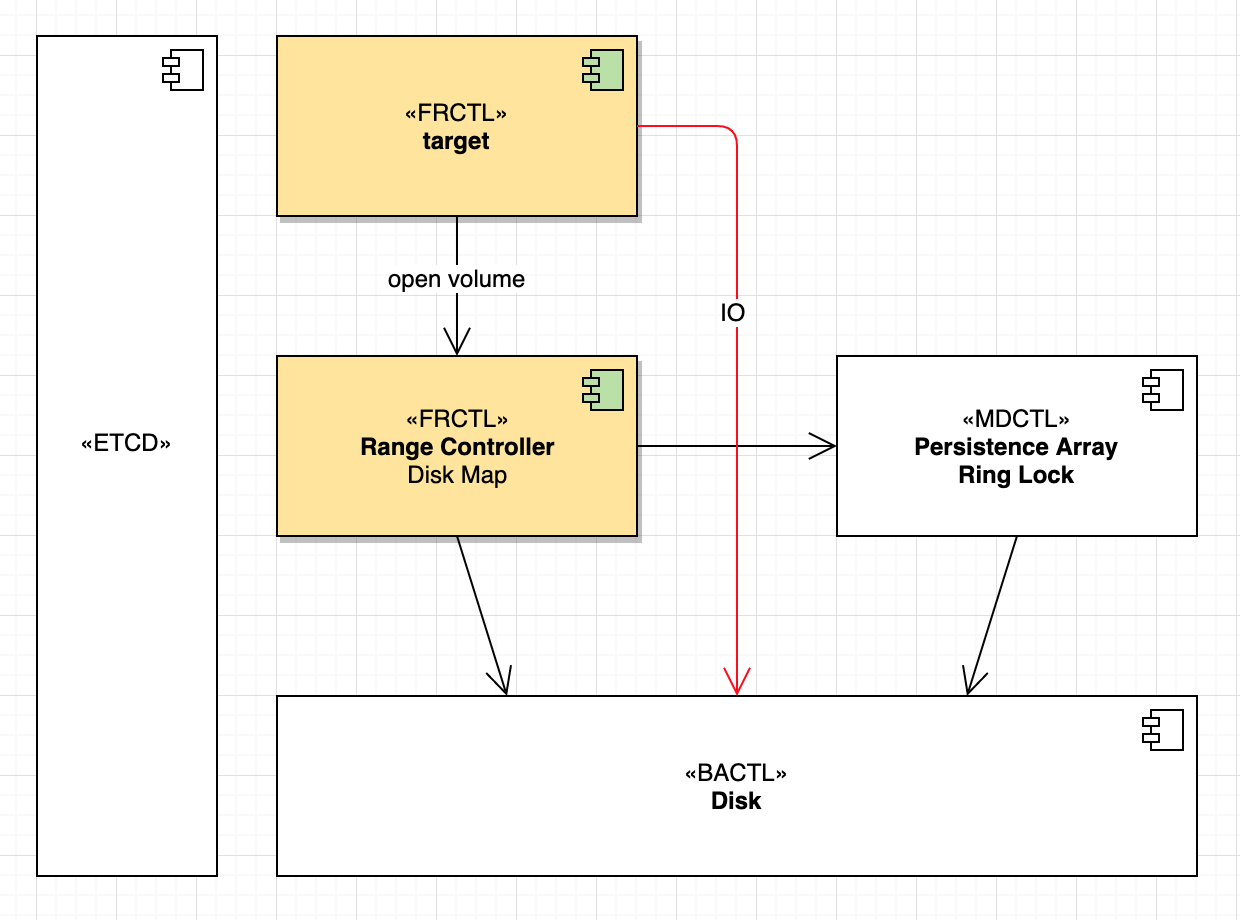
\includegraphics[width=11cm]{../imgs/modules.png}
\end{center}

target到bactl,有两条路径,视是否通过range ctl而定。如果不通过range ctl(rangectl bypass),数据流可直达后端存储,
实现控制流和数据流分流的目的。同时降低了转发成本。

问题集:
\begin{enumbox}
\item 为什么range ctl和mds是分离的进程?
\item vss是否必要?
\item ***
\item io路径是什么?
\item 副本一致性是如何实现的?
\item IO和Recovery之间如何同步?
\end{enumbox}

\subsection{FRCTL}

target如何与分布式卷相连?

vss包括4个range,range包括4个pa,pa包括固定数目的chunk。pa和chunk都是4M大小。
\todo{vss是否必要}vss是否必要,还是增加了设计复杂度?

token是向range ctl获取的,粒度为chunk。range ctl上每个chunk维护有token计数器。

token里包含了每个副本的位置信息,这是向mds请求得到的。

client并不与mds直接通信。分离fr和mds为两个进程,一是可以指定不同的core;二,便于debug。

\begin{center}
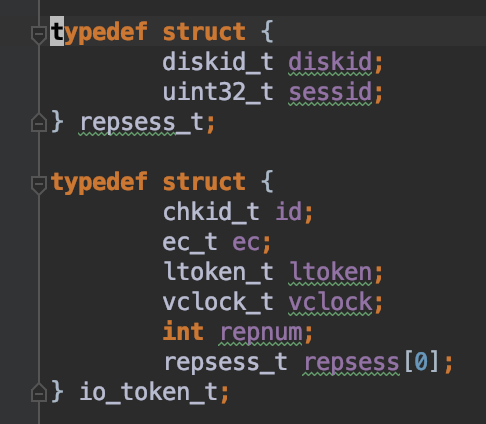
\includegraphics{../imgs/token.png}
\end{center}

range ctl和mds都在hash ring上。都采用了hash机制来定位目标节点。
所以\hl{有两个hash ring:range ctl和mds}。两个ring都通过mds master来维护。
ring的节点结构是什么?node and core?
\begin{center}
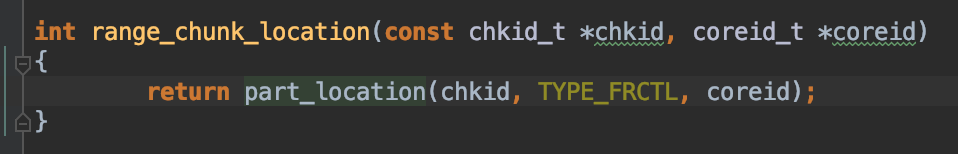
\includegraphics[width=11cm]{../imgs/chunk-location.png}
\end{center}

partition是range ctl和mdctl共用模块。range ctl目前归属frctl。

lease机制目前没用,如果需要把range ctl放置到session所在的位置(一个volume的所有range都在一个节点上?),
可以选用lease机制,而不用dht机制。怎么理解session?

一旦ring结构发生变化,会有什么影响?SSAN通过epoch来管理ring结构的变化。

ring上节点负载均匀性如何?

ring lock有什么用?在mds master上维护状态,处理ring发生变更的情况。
是否可通过引入epoch实现同样的功能?

GFM?解决全局同一视图的问题。

如何识别和处理stale消息?

\subsection{MDCTL}

hash ring上有一个节点充当master角色。如何选主,如何保持其唯一性?
通过etcd lock实现。

\subsection{BACTL}

diskid是全局的,在etcd上有目录。

\subsection{Driver}

diskmd磁盘访问接口,支持libnvme驱动。

需要管理物理内存,如hugepage和memory pool。

NVMe/RDMA需要访问物理内存。

\section{资源}

从\hl{资源的生命周期模型}开始思考。资源包括:\hl{集群、节点、core、磁盘、pool、volume、snapshot}等,以及内部资源。

ERD

\subsection{Cluster}

\subsection{Node}

Node是Process、Core、Disk等资源的合集。利用Core的方式是个亮点。

增删节点是重大事件

\subsection{Disk}

Disk导出,分配过程可以进行全局调度。

调度器位于md ctl。md ctl负责管理chkid到disk id的映射关系。
\todo{diskid类型}diskid采用16bit整数是否太小?

diskmap.c,不宜放入bactl。bactl所有API都带diskid,针对单盘进行。

怎么做到每个副本属于不同的节点的呢?

如何管理diskmap的版本呢?

\hl{数据分布的均匀性}: 节点和磁盘两种粒度

tier and cache?

负载均衡

\subsection{Pool}

\subsection{Volume}

\begin{enumbox}
\item TP
\item Recovery
\item Balance
\item QoS
\item ***
\item EC
\item Dedup
\item Compress
\item ***
\item RC
\end{enumbox}

\subsection{Snapshot}

如何共享底层对象?

consistency group

分析各种操作的复杂度,包括空间和时间。

\hrulefill

平安科技:可写快照

与COW平列实现ROW?

快照占据底层volume空间共享?

COW的问题
\begin{enumbox}
\item 影响写性能
\item Rollback慢
\item clone卷慢,scan snap tree。snapshot也可执行flatten
\end{enumbox}

snap头包含什么指针?

快照卷与物理卷什么对应关系,

映射表的管理粒度,是chunk还是page?范围,是全局还是私有?

COW一次读,两次写

ROW一次读,一次写

\hrulefill

SSAN的snapshot实现。

ROW,两层元数据?

vol id发生变化,凡是依赖于vol id的都需要进行适配。

\section{数据}

\subsection{ETCD}

\subsection{卷的元数据}

两层元数据,etcd指向顶层对象。每个对象属于一个卷,
因为不是一般的对象系统,\hl{在快照的情况下,无法直接共享}。

% \chapter{ETCD}

/opt/fusionstack/etcd


etcdctl ls -r


\chapter{模型}

\begin{tikzpicture}[show background grid]
    \begin{class}{Disk}{6, 0}
    \end{class}
    \begin{class}{Pool}{6, 2}
    \end{class}
    \begin{class}{Volume}{6, 4}
    \end{class}
    \begin{class}{Host}{6, 6}
    \end{class}
    \begin{class}{Cluster}{0, 2}
    \end{class}
    \begin{class}{Snapshot}{0, 4}
    \end{class}

    \composition{Cluster}{pools}{1..*}{Pool}
    \composition{Pool}{disks}{1..*}{Disk}
    \composition{Pool}{volumes}{1..*}{Volume}
    \composition{Volume}{mapping}{*..*}{Host}
    \composition{Volume}{snapshots}{1..*}{Snapshot}
\end{tikzpicture}

\section{Cluster}

整体

\section{Pool}

把物理节点划分为不同的保护域,一个卷的所有数据只出现在一个保护域内。卷可以跨保护域进行复制和迁移。

默认一个,包括所有节点。

% 保护域是物理节点的划分,存储池是存储介质的划分。每块盘只能出现在一个存储池里。

Pool: 逻辑容器

故障域有粒度之分,如磁盘,节点,机架,机柜,数据中心。

存储池内,要满足故障域规则:一个chunk的不同副本,分布在不同的故障域内。\label{rule:faultset}

在初次分配,再平衡和恢复等过程中,都需遵循这些规则。

\begin{tcolorbox}

可以参考ceph的CRUSH实现。bucket和device定义了集群的物理拓扑结构,rule定义了数据存取规则,
pool上关联rule,从而定义了pool中卷数据的放置规则。设备即OSD,对应一个物理磁盘。

***

存储池可以取代保护域,定义所有对象的存放位置是一个节点集。

***

存储池可以用来实现tier cache。重定向IO到cache pool。

***

统一概念:保护域,故障域,存储池,pool。Consistency Group不同于pool,与物理存取无关,
而是卷的逻辑集合,卷可以来自不同的pool。

\end{tcolorbox}

与存储池有什么同和异?存储池可以看做关联了磁盘的pool,可以看做pool的子类。

属性:
\begin{enumbox}
\item 配额
\item 复制类型:副本 OR EC
\item 磁盘列表
\item 定义精简池
\item 存储池上可以指定卷的副本数
\item \hl{有足够的故障域,且不同故障域配置一致的资源量}
\end{enumbox}

操作:
\begin{enumbox}
\item 创建
\item 删除
\item 扩展(添加磁盘到\hl{已存在的存储池},该映射关系持久化到本地,同步到admin节点)
\item 缩容(从存储池中移除磁盘,引发数据重建过程)
\item \hl{自动或手动按磁盘速率进行存储池分级划分}
\item 不同存储池之间,卷的复制
\item 不同存储池之间,卷的迁移,可在线或离线
\item 存储池级别的统计信息
\end{enumbox}

% 存储池是disk的集合,与节点无关。但disk所在的节点构成存储池的节点列表,不同存储池的节点可能覆盖。

存储池下,可以创建volume。没有关联磁盘的存储池,不能创建卷。

\hl{chunkid到磁盘物理位置有两级映射:chunk的副本节点列表,节点内chunkid到物理地址的映射}。

在为卷分配chunk的时候,需要确定各个副本的物理存储位置。当前实现是返回不同副本的节点列表。
如果指定了存储池,就需要在存储池所在的节点范围内进行分配。同时要满足故障域和数据均衡规则。

\begin{tcolorbox}
移动采集中存储池要求,相比于目前的逻辑pool,更多是一种设计上的退步。
存储虚拟化的目标,是物理位置无关。我们可以基于逻辑容器,实现基于策略的管理。
所以,\hl{从实现层面,要保留当前pool的功能,按照系统配置确定pool的类型}。
\end{tcolorbox}

% 存储池内,要满足故障域规则(\ref{rule:faultset})

步骤:
\begin{enumbox}
\item 创建pool,但此时不能创建pool的元数据chunk,因为还没有绑定磁盘(需要一全局的地方,存储pool名字)
\item 添加磁盘到pool,通知admin节点
\item 当在pool下面创建卷的时候,前提条件是已准备好磁盘,生成pool元数据chunk(位于同一pool里)。
\end{enumbox}

pool元数据chunk必须位于自己的存储池内,如果分布在不同的存储池,不满足故障域条件。

pool引导信息可以存在rootable里。

\section{Volume}

属性:

操作:
\begin{compactenum}
    \item rename
    \item resize \info{在线扩容}
    \item mv
    \item copy \change{全量拷贝/增量拷贝} \change{跨存储池拷贝} % change不能出现在box里
\end{compactenum}

\section{Snapshot}

snapshot隶属于卷,无卷则无快照,快照组织成快照树,其中有且只有一个快照是可写快照,即卷的写入点。

\section{Mapping}

数据隔离/ACL,数据保护

卷对主机的可见性。一个卷只有映射给了某主机,才可以被该主机访问。


\section{Consistency Group}

一致性卷组

\begin{shadequote}
Consistency Groups could be useful for Data Protection (snapshots, backups) and
Remote Replication (Mirroring).

The Mirroring support will allow to setup mirroring of multiple volumes in the
same consistency group (i.e. attaching multiple RBD images to the same journal
to ensure consistent replay).

There is already an interest to implement this functionality as a part Mirroring feature:
http://tracker.ceph.com/issues/13295

The snapshot support will allow snapshots of multiple volumes in the same
consistency group to be taken at the same point-in-time to ensure data
consistency.
\end{shadequote}

\chapter{Pool}

\section{接口}

\begin{enumbox}
\item pool create
\item pool rm
\item pool info or stat
\item pool list all
\item pool add disk
\item pool remove disk
\item pool list disk
\end{enumbox}

\section{迁移}

离线/在线迁移

不改变卷ID。卷ID和chunkid集群内唯一,迁移过程中保持不变。

怎么判断一个卷是离线还是在线?有无访问者。target上的链接数,
每个卷的volume\_proto都有一个connect\_list。

\begin{lstlisting}[language=bash,frame=single]
# lich.inspect --connection /iscsi/p1/v1
\end{lstlisting}

基于快照实现存储池的迁移和复制。相当于clone了新卷,chunkid皆发生变化。


\section{复制}

\chapter{Volume}

卷可以建模为状态机,不同状态允许不同的操作,按条件在不同状态之间切换。

\section{属性}

\begin{lstlisting}[language=c,frame=single]
typedef struct {
        fileid_t id;
        uint16_t magic;
        uint16_t repnum;
        uint64_t snap_rollback;
        uint64_t snap_version;
        uint64_t reference;         //clone reference
        uint32_t attr;
        int32_t  priority;
        uint32_t __pad__[4];

        uint64_t size;
        uint32_t mode;
        uint32_t uid;
        uint32_t gid;
        uint32_t ctime;
        uint32_t mtime;
        uint32_t btime;
        uint32_t atime;
} fileinfo_t;
\end{lstlisting}

卷是ServerSAN核心对象,是pool,snapshot,mapping和cg的中心。

卷的属性记录在L1 chunk的fileinfo段。fileinfo段是vol info区的第一个段。

\subsection{大小}

目前,卷的元数据由两级组成:L1,L2。L1只有一个chunk,每个chunk有8000个槽位。每个槽位指向一个L2 chunk。
L2 chunk有16000个槽位,每个槽位指向一个raw chunk。所以,最大卷大小约为$122TB = 8000 \times 16000 \times 1MB$。

为了支持更大的卷,需要扩展此结构,把L1扩展到多个chunk。改变会影响到:
\begin{compactitem}
\item 加载table1 (加载多个chunk,记录每个chunk的chunkinfo信息)
\item table1的各项操作
\item 遍历卷的chunk
\item 数据恢复过程
\item migrate
\item copy
\item snapshot clone,需要copy L1 chunk
\item ...
\end{compactitem}

L1 chunk:vol.xxx.0, vol.xxx.1, vol.xxx.2。其中,vol.xxx.0的chunkinfo记录在pool。
\hl{vol.xxx.1等chunkinfo记录到vol.xxx.0里info区的第二个块,并需记录其个数}。动态加载。

父:raw和subvol的父chkid为vol.xxx.0,vol.xxx.1的父chkid也为vol.xxx.0。vol.xxx.0的父chkid为所在pool的chkid。

缺页中断:从上到下检查。创建chunk的时候,先检查L1 chunk是否存在,然后检查L2 chunk是否存在。
不存在,则创建。在以下过程会改变卷的数据结构树:
\begin{compactitem}
\item \verb|__pool_proto_mkvol|
\item \verb|volume_proto_load|
\item \verb|volume_proto_chunk_pre_write|
\item \verb|__volume_proto_chunk_allocate|
\end{compactitem}

\begin{lstlisting}[frame=single]
lichbd write /iscsi/p1/v1 hello -o 280375465082880
lichbd cat /iscsi/p1/v1 -o 280375465082880 -l 5
\end{lstlisting}

chunk allocate开销较大,即要申请磁盘空间,也涉及记录元数据到父节点。

遗留问题:
\begin{enumbox}
\item lich.inspect --stat极慢 (统计,load)
\item 分析内存占用量
\item clone
\item recovery
\item balance
\item 回收空间
\end{enumbox}

\subsection{副本数}

\section{操作}

\begin{enumbox}
\item create
\item rm
\item ls
\item info
\item resize
\item rename
\item mv
\item copy (read/write)
\item migrate (move all chunk)
\item duplicate (snapshot-based: clone/flatten)
\item import
\item export
\item mapping
\item \hl{IO}
\end{enumbox}

\subsection{create}

\subsection{rm}

显式回收空间

分为两阶段:标记和回收。先把卷移入/system/unlink,有后台异步线程负责回收。

相关源文件:
\begin{compactitem}
\item pool\_rmvol.c
\item rmvol\_bh.c
\end{compactitem}


\subsection{QoS}

token bucket。IOPS与block size相关,两者乘积等于带宽。
如果各层发生IO聚合,则在流量守恒的情况下,显示IOPS有所不同。

IOPS必须假定一定的block size。

\chapter{快照和克隆}

\chapter{任务管理}

后台任务处理,或事件驱动,或定时器驱动。
线程或线程池按一定方式组织,采用actor或csp并发编程模型。

为了在集群级别进行控制,采用主控、或定向策略,提供可控性和性能。
Nutanix的Mapreduce并行执行模型。

\section{平衡}

\subsection{控制器平衡}

每个卷到core的映射是可计算出来的,可按core逐个进行平衡。
先处理core hash等于0的卷,依次类推,同时使迁移量尽量少。

以上算法假定每个卷都是等价的。如果卷的大小和负载不同,目前方案难以做到真正的平衡。

\subsection{数据平衡}

\begin{enumbox}
\item 按pool划分
\item 每个pool,分布在多个节点上,每个节点可得其磁盘利用率
\item 符合move条件的raw chunk,确定其新的副本位置集
\item 迭代执行,重新评估
\end{enumbox}

\section{恢复}
活动的可追踪性,比如scan阶段的时间,是分析系统行为至关重要的指标。
做到重要事件有迹可查,可以审计。

采用SEDA架构组织处理过程,分scan和recovery两阶段,边扫描,边恢复。
pipeline

QoS,参考操作系统的进程调度(MLFQ),网络的流量控制,多级反馈队列等。

采用强化学习的思路动态调整控制参数。

区分节点故障和磁盘故障,磁盘故障时可以利用sqlite信息,直接扫描。

移除磁盘时,调用\verb|md_chunk_set|,设置该磁盘上所有chunk的chkinfo的对应副本状态为\verb|_S_CHECK__|。
恢复过程,根据chkinfo的副本状态,判断是否需要恢复。如果需要恢复,调用\verb|md_chunk_check|。

\verb|md_chunk_set|过程开销较大,故感知磁盘故障的延时较长。\hl{把副本状态持久化到chkinfo里,是否真的必要}?

\hl{节点下线}触发怎么样的过程? \verb|network_connect1|。

故障域规则

单个磁盘

单个节点

单个机柜

重建性能

不中断IO

\subsection{需求}

恢复性能和Qos机制。

控制系统后台数据恢复进程所占用的带宽和 IO 处理资源,提供多种数据恢复的优先级策略。

至少提供优先前端应用或优先数据修复这两种优先级策略。在优先前端应用的策略中,数据
修复仅在资源较空闲时进行;在优先数据修复策略中,后台恢复以最快速度完成,
但卷仍然在线保持可用,仅性能有所降低。

作为作业管理,展示恢复进度,关键参数和资源消耗情况。

当有app io时,恢复性能变慢,原因是任务调度吗?

故障恢复过程中,数据迁移和写入,遵循 tier或 cache策略,优先写SSD,每节点SSD数量有限,
在同时承担业务访问情况下,极易成为瓶径,本次实测恢复数据每节点 10MB/s 以下,
恢复QoS无法体现作用。节点中机械盘不能并发参与恢复。

恢复QoS当前每节点分别命令处理,需要换一种全局可控的方式(例如带宽或网卡百分比,这部分产品先找资料进行参考)

rebalance 是否也是优先写SSD? 应与恢复相同策略,不设置QoS情况下,
应最大限度利用全部机械盘进行并发数据恢复,减少或不占用SSD资源。

\subsection{相关特性}

恢复策略与磁盘热插拔,磁盘漫游相关。

\subsection{设计}

至少可以设定两个等级:恢复优先,或应用优先。至于恢复线程数,等待时间,更多是实现细节,用户很难自己设定。
所以,需要更高级的控制语义。

目标,偏离,反馈,调节,达到控制的目的。分析上下限,临界情况,执两用中。

串行恢复一个chunk的性能,并发情况下的加速比(串行是基准)。

在不受限制的情况下,先优化到最大性能,能否达到硬件瓶颈?

需要有约束的机制和策略。控制并发度和等待时间。

在每个节点上运行恢复线程,分两个阶段:
\begin{itemize}
\item 扫描,确定需要恢复的chunk
\item 恢复,多线程执行
\end{itemize}

每个节点只处理属于本节点的数据,即主副本位于本地节点。从sqlite扫描chkid,逐个检查其repnum,
是否与fileinfo一致,如果不一致,追加到一临时文件
\begin{itemize}
\item chkinfo.repnum是实际副本数(需要进一步查看各副本的真实状态)
\item fileinfo.repnum是目标副本数
\end{itemize}

控制参数:
\begin{itemize}
\item 功能开关
\item 数据恢复的最大带宽(\hl{token bucket 填充速率})
\item 线程数
\item 线程处理完一个chunk后的sleep时间
\end{itemize}

前端优先对应的控制参数是什么?恢复优先对应的控制参数是什么?自定义QoS?

系统级别的配置信息存在哪儿?结构采用KV,有几种方案可供选择:
\begin{itemize}
\item etcd           增加了外部依赖性
\item ZK             增加了外部依赖性
\item /config/       lich运行后,方可访问
\item /dev/shm/lich4 非持久化
\end{itemize}

单次扫描的条目不宜过多。

\subsection{实现}

配置目录:/dev/shm/lich4/nodectl/recovery

\begin{itemize}
\item immediately       功能开关
\item interval          恢复任务的时间间隔
\item thread            工作线程数
\item suspend
\item qos\_maxbandwidth 设置最大带宽
\item qos\_sleep        设置sleep多少豪秒
\item qos\_cycle        设置计算带宽的时间间隔
\item info              输出结果
\end{itemize}

md\_chunk\_getinfo

md\_chunk\_check

\subsection{测评}

从串行到并行

\begin{itemize}
\item 各阶段时间
\item 磁盘利用率
\item 并发度
\end{itemize}

为什么在有前台IO的情况下,性能严重下降?

\subsection{运行}

\begin{tcolorbox}
    自动触发:Recover 每10分钟执行

    手动触发:echo 1 > /dev/shm/lich4/nodectl/recovery/immediately
\end{tcolorbox}

\section{GC}

chunk

\section{Clock Merge}

\section{监视存储池状态}

由admin节点执行

\section{删除卷}

任务规范放入etcd更合适,避免因为ENOSPC,导致删不了。

\section{删除快照}

\section{回滚快照}

\section{flatten}

%\section{HSM}

%分层存储管理
%\begin{itemize}
%\item \verb|__volume_ctl_analysis_init|
%\item \verb|replica_hsm_init|
%\end{itemize}

%\section{SSD Cache}

%\begin{itemize}
%\item \verb|__flush_create|
%\end{itemize}


\chapter{优化项}

\section{时间优化}

\begin{itemize}
    \item localize
    \item auto tier
    \item ssd cache
\end{itemize}

\section{空间优化}

\begin{itemize}
    \item 精简配置 (Thin provisioning)
    \item EC
    \item Dedup
    \item Compress
\end{itemize}



\chapter{QOS}

\section{概述}

学习的方法:
\begin{enumbox}
\item \hl{对标}:行业的标准做法是什么?
\item 如何才能更好地学习?
\item *
\item 先选出几篇经典论文,顺藤摸瓜,建立相关的知识体系。
\item 与专业人士交流,获取有价值的线索。
\item 还需要主动去悟,提问、消化、守破离,推陈出新
\end{enumbox}

参考网络QoS,存储QoS的核心算法与网络QoS相同。

集中式控制、分布式控制

排队论

态势感知?

在高IOPS的情况,QoS的开销过大,极大地拉低了性能,这是不可接受的。

每次请求都要获取一次时间,是不是必要的?

\subsection{参考}

\begin{enumbox}
\item OS中进程、线程调度算法
\item Disk IO调度算法
\item VM IO调度算法
\item Network QoS and Storage QoS
\item TCP/IP
\item iSCSI
\item SPDK QoS
\item Ceph dmClock
\item SolidFire QoS
\end{enumbox}

\section{算法}

采用了两种曲线

开放控制参数

比较指标:理论和实测值的距离,\hl{也可以考虑夹角的大小}。\change{距离函数}

底层采用token bucket,需要能容忍一定的jitter。

在调度器内加入QoS控制逻辑的设想: 每个core调度器对应一个或若干卷控制器。基于优先级队列,由core线程处理队列(scheduler队列?)。
每个卷控制器在对应的scheduler上注册自己的队列(IO任务、恢复任务)。 \hl{core上的每个卷,向scheduler注册自己,从而实现解耦}。
调度器不仅可以处理单个卷的QoS,也可以处理多个卷的QoS。

\hl{队列和线程}往往紧密结合为一体,参见SEDA、actor。

\hl{多mode调度器},根据实际负载条件动态地调整调度器策略。

何时从请求队列移入调度队列是QoS调度器的中心任务。

% \section{Quota}


% \chapter{企业级特性}

\section{Security}

iscsi CHAP认证

\section{QOS}

token bucket

\change{距离函数}


\section{Quota}

\section{Multipath}

\section{DR}

snapshot

io journalling

\section{CDP}

\chapter{LSV}

现有Lich raw卷,存在性能问题,COW快照也不便于扩展。所以实现了Log structured Volume,
转化随机IO为顺序IO,基于其上,实现了ROW快照。

特别要注意的是,实现中应着力避免顺序IO随机化,会引起IO放大,从而极大地降低性能。


\section{Volume}

Volume模块负责空间管理。提供malloc/free接口,也可批量分配和回收。采用bitmap和free list多种管理方式。
freelist充当分配缓冲区的角色,可持久化,也可不持久化。

lsv-lich raw-disk的chunk空间存在两级映射关系,会影响到读写性能。

底层空间宜按固定大小的段来组织。每个段空间管理的开销是固定的。
目前支持两级存储分级:
\begin{tcolorbox}
    \begin{multicols}{2}
        \begin{itemize}
            \item 0:ssd
            \item 1:hdd
        \end{itemize}
    \end{multicols}
\end{tcolorbox}

\section{Bitmap}

Bitmap更合适的叫法是页表,与操作系统里的页表类似,负责虚拟地址到物理地址的映射关系。Bitmap有两层:L1和L2,
按类似页表的方式组织。和Log层数据一起,构成三层。

L1是Bitmap的头部,大小固定,属于卷或快照私有。L2按需分配,在快照之间共享。在Clone的情况下,会涉及跨卷读。

通过Bitmap层,支持快照的全部特性,多个快照构成快照树。快照树分两种方式展示:树状或列表。

\section{Log/Chunk}

底层物理空间,划分为固定大小为1M的数据块,进行统一管理:分配/释放。

在Volume模块之上做了简单封装,表示卷的数据,Bitmap表示卷的元数据。在覆盖更新的情况下,Bitmap指向新的数据页,
导致原来的数据页失效,可以回收。在有快照的情况下,会变得较为复杂。

Log模块无需要持久化的信息。

在Lich卷空间映射到磁盘的时候,目前实现为一个随机过程。\textcolor{red}{磁盘的1M随机和顺序,差别较大}。

\section{WBuf}

Wbuf有两个序列:WAL和Wbuf的提交序。在wbuf中读出的最新数据和提交后通过bitmap+log读取的数据,应该一致。

IO内,LBA不同,无冲突,页序;IO间,LBA可能相同,有冲突,需要串行化。

\section{RCache}

多级缓存机制,需要注意针对多种读场景进行优化,如顺序读。因为经过虚拟页表映射,虚拟地址空间和物理地址空间,顺序可能是交叉的。
应着力避免出现顺序变随机导致读放大的情况。

预读很重要,也比较困难,需要构建学习模型。

\section{GC}

log功能单一化,gc模块独立出来。gc要解决的问题有二:
\begin{enumerate}
    \item 跟踪所有log
    \item 在所有log中,根据一定策略(qos),选择回收价值最大者进行回收
\end{enumerate}

目前的实现,是局域的解,而不是全局最优解,是bottom-up的分代垃圾回收器。可增量并行执行,与前台赋值器需要同步机制。
回收器和赋值器需要读写barrier。

优化GC Check过程:每一页的信息,只会出现在部分的bitmap记录里,与快照树的拓扑结构有关。
在创建快照时,分配snap id。 snap id组织成单调递增的序列。如果中间没有删除或rollback操作,
很容易定位到某页所属的快照点。经过rm或rollback之后,情况有所不同,但依然有迹可循。

\section{Recovery}

正常关机的情况下,各个模块会flush必要的数据,下次启动的时候,load出来即可。

异常关机的情况下,各个模块没有机会flush数据,导致丢失部分内存状态信息。
这样,在下次启动的时候,需要执行恢复过程。

需要flush数据的模块有:
\begin{itemize}
    \item Wbuf
    \item GC
    \item Volume
\end{itemize}

提出几个问题:
\begin{tcolorbox}
\begin{enumerate}
    \item 正常关机时,需要flush什么信息?
    \item 恢复过程,从X恢复出Y,X是什么?Y是什么?(X是日志,Y是最新状态)
    \item 怎么理解提交等基础操作?
    \item 恢复的性能如何?如何通过检查点机制改善恢复性能?
\end{enumerate}
\end{tcolorbox}

针对以上问题,每个模块的恢复机制有所不同,但分析方法具有通用性。

\subsubsection{Volume Recovery}

 $U = (A - B) + C + D$

tail标记了可见空间,可见空间=已分配+可分配(free list)。free list组织成内存和磁盘两部分。flush时,需要持久化freelist的内存部分。

在调用malloc和free接口的时候,会同步更新用于空间管理的bitmap。为1的为已分配,为0的为可分配,这个关系总成立。

为了支持批量malloc和free接口,引入dirty page bitmap,类似于GC中提到的卡表,可以实现\textcolor{red}{多次更新,一次提交}的设计模式。

主要操作:
\begin{tcolorbox}
\begin{itemize}
    \item malloc操作:依次从C,D,U里取可用chunk。
    \item free操作:把释放的chunk放入C,如果C满,则转化为D。
\end{itemize}
\end{tcolorbox}

这里的提交操作可以理解为:C转化为D的过程,并没有记录检查点。
所以恢复操作,要全扫描bitmap,从bitmap重建C和D。

\subsubsection{GC Recovery}

GC recovery过程可以理解为:从gc bitmap重建内存状态。

所有的log,分为两部分:old storage和bitmap。bitmap相当于journalling。进入check queue的logctrl,先登记到bitmap。
在提交时,即从heap移入old storage时,清除/注销相应的bitmap项。

\subsubsection{Wbuf Recovery}

谁充当了日志的角色?在wbuf模块很明确,有专门的WAL。写入阶段登记,commit阶段回收。

\section{LSV测试}

LSV(\textcolor{red}{Log Structured Volume})基于Lich原生卷,实现了日志结构的卷格式,支持快照的各种操作。

相对于Lich原生卷,LSV有几点优势:
\begin{tcolorbox}
    \begin{itemize}
        \item 转化随机IO为顺序IO,混合存储情况下有更高性能
        \item 实现为ROW快照,zero-copy快照,\textcolor{red}{支持快照树}
    \end{itemize}
\end{tcolorbox}

LSV的关键过程:
\begin{tcolorbox}
    \begin{description}[style=nextline]
        \item [写] 写入wal和wbuf后,即可返回。wbuf积聚到1M时,提交log+bitmap后台异步任务。
        \item [读] 从wbuf读取最新数据,如果没有命中,则依次从rcache,bitmap+log读取。
        \item [GC] 垃圾回收,后台异步任务,按一定策略,回收无效页。
        \item [重启] 分两种情况,正常和异常情况。正常情况下会刷新内存状态,重启时直接加载即可;异常情况下,进入recovery过程。
    \end{description}
\end{tcolorbox}


LSV测试,主要分为功能,正确性和性能几个方面,\textcolor{red}{正确性和性能按标准测试用例}执行即可。下面列出一期测试计划。

\subsubsection{GIT分支}

lsv\_pipeline

\subsubsection{特性}

%\begin{tcolorbox}
\begin{lstlisting}[language=bash,frame=single]
# 创建LSV卷:
lichbd vol create p1/v1 --size 100Gi -F lsv -p iscsi

# 快照功能,与原来一样,部分命令示例:
lichbd snap create p1/v1@snap1 -p iscsi
lichbd snap create p1/v1@snap2 -p iscsi
lichbd snap ls p1/v1 -p iscsi

# 暂不支持flat操作

\end{lstlisting}
%\end{tcolorbox}

\subsubsection{性能/正确性测试清单}

\begin{itemize}
    \item 与lich原生卷全面的性能对比
    \item 资源利用率(包括磁盘,内存)
    \item 系统启动时间
    \item 重启系统的恢复过程
    \item 存储分层
    \item 扩展到多卷
\end{itemize}

\subsubsection{注意事项}

\begin{itemize}
    \item 日志满:/opt/fusionstack/log/lich.log (echo 5 > /dev/shm/lich4/msgctl/level)
\end{itemize}


\chapter{iSCSI}

\section{IQN}

关于iqn的不变性,iqn是卷的公开标示,供上层应用引用该卷。改变iqn,需要通知依赖于iqn的应用,做出相应的改变。

回到lich的情况,iqn包含了路径部分:<pool\_name>.<image\_name>,跨存储池迁移,rename等操作会改变路径部分。

问题: 可否用卷的volid作为iqn的一部分,替代path,同时保证volid在各种操作下具有不变性?

ceph的做法:
\begin{compactenum}
\item rbd访问方式,用的是路径。
\item 通过tgt提供iscsi服务时,通过tgt配置项建立iqn到path的映射
\end{compactenum}

\begin{lstlisting}[frame=single]
<target iqn.2014-04.rbdstore.example.com:iscsi>
    driver iscsi
    bs-type rbd
    # Format is <iscsi-pool>/<iscsi-rbd-image>
    backing-store iscsi/iscsi-rbd  
    initiator-address <clients address allowed>
</target>
\end{lstlisting}

\section{CHAP}

In function \verb|ns_build_auth_chap|
\begin{compactitem}
\item \verb|lich_system_username|
\item \verb|lich_system_password|
\end{compactitem}

\section{白名单}

\begin{compactitem}
\item \verb|is_connect_allowed|
\end{compactitem}

没有设置ip或initiator,默认拥有全部权限,不符合白名单语义,最小权限原则。

xattr用于保持ip或initiator白名单,如果很长,则溢出。
需要找到更合适的存储方式。

\section{Initiator}

\begin{lstlisting}[language=bash,frame=single]
echo 2 > /sys/block/sdd/device/queue_depth
cat /etc/iscsi/initiatorname.iscsi
\end{lstlisting}

\chapter{设计}

设计在解决关键问题的同时,要降低实现,测试和维护的复杂度。

加强测试,通过重构降低复杂度。

分解问题,界定边界,降低复杂度

设计的基本原则

分离机制和策略,接口和实现

性能依赖于设计,在一定的设计下,取决于实现。

性能优化手段:并行,聚合,缓存等,根本在于设计,控制复杂度。

识别实体和关系,ERD,DFD等,FSM是机器语言。

核心概念:
\begin{compactenum}
\item 存储池/目录
\item 卷
\item 快照
\item 主机映射
\end{compactenum}

core thread边界,core\_request进入。

分布式副本一致性:clock版本机制,msgqueue离线消息处理。

性能:并发,聚合和cache等

元数据管理,非计算而来

快照树的实现

后台任务统一管理,包括:
\begin{compactenum}
\item recovery
\item balance
\item vol rm
\item snap rm
\item snap rollback
\item snap flat
\end{compactenum}

架构问题:
\begin{compactenum}
\item 元数据管理成本
\item 支持大容量卷
\item 支持ROW快照树
\item 诊断流程和工具
\item 性能profile
\end{compactenum}

\section{故障域}

对任一存储池,设故障域数为M,副本数为N,

当M>=N时,每个故障域内一个副本,随机分布;
当M<N时,
- 策略1,每个故障域内一个副本
- 策略2a,剩余的副本按策略1进行,直到写完所有副本数
- 策略2b,不写剩余副本

按策略2a:

case 1:故障域为2,副本数为3,则副本在故障域的分布为(2,1)或(1,2)
case 2:故障域为1,副本数为3,则副本在故障域的分布为 3

按策略2b:

case 1:故障域为2,副本数为3,则副本在故障域的分布为(1,1)
case 2:故障域为1,副本数为3,则副本在故障域的分布为(1) (副本数不能少于2个,分配失败)

同时,恢复过程须按以上故障域规则进行自动校正!!!

\section{存储池状态}

\begin{compactenum}
\item 不可用
\item 磁盘空间不足/READ ONLY
\item 降级
\item 正常/健康
\end{compactenum}

\section{诊断方法}

对需要改进的流程进行区分,找到最有潜力的改进机会,优先对需要改进的流程实施改进。如果不确定优先次序,企业多方面出手,就可能分散精力,
影响6σ管理的实施效果。业务流程改进遵循五步循环改进法,即DMAIC模式:

\begin{compactenum}
\item 定义[Define]——辨认需改进的产品或过程,确定项目所需的资源。
\item 测量[Measure]——定义缺陷,收集此产品或过程的表现作底线,建立改进目标。
\item 分析[Analyze]——分析在测量阶段所收集的数据,以确定一组按重要程度排列的影响质量的变量。
\item 改进[Improve]——优化解决方案,并确认该方案能够满足或超过项目质量改进目标。
\item 控制[Control]——确保过程改进一旦完成能继续保持下去,而不会返回到先前的状态。
\end{compactenum}

信息有多级:USE。诊断问题依赖于结构化的诊断方法PAT,解决问题也是,构建知识图谱。

欲分析问题,必分析事物发展的完整过程,包括每个参与者的生命周期模型,参与者之间的相互作用。

\section{检查清单checklist}

先宏观,后微观,致广大而尽精微

\begin{compactenum}
\item 集群健康情况
\item 数据一致性检查
\item 硬件
    \begin{compactenum}
    \item 磁盘
    \item 网络
    \item 内存
    \item CPU
    \item 操作系统
    \end{compactenum}
\item LICH
    \begin{compactenum}
    \item 后台任务,包括恢复,删除,快照后台任务等
    \item 日志
    \item core
    \end{compactenum}
\end{compactenum}

\chapter{实现}

\section{Schedule}

不能支持嵌套task,用pre yield变量来控制。

\section{内存}

提供什么接口,三种生命周期范围、持久性:
\begin{easylist}[itemize]
& 常驻
& session
& IO
\end{easylist}


使用场景
\begin{easylist}[itemize]
    & core private memory
    & sche\_task
    & RDMA
    & buffer\_t
    && libnvme
    & little object
    & ring
\end{easylist}

采用buddy算法管理连续内存分配

动态化

用面向对象的方式处理,每个core对应一个MR对象。public的也是如此。

每个对象内嵌一个buddy对象管理hugepage的分配、释放。
另外,从core的MR里,利用buddy算法分配连续内存,用于ring等小对象。

禁止在一个core内malloc,由另外一个core进行free。

怎么抽象一般内存和hugepage-based内存?

抽象出head,core和public重用代码。第一选择head,第二执行head的操作。

\subsection{buffer}

\begin{center}
    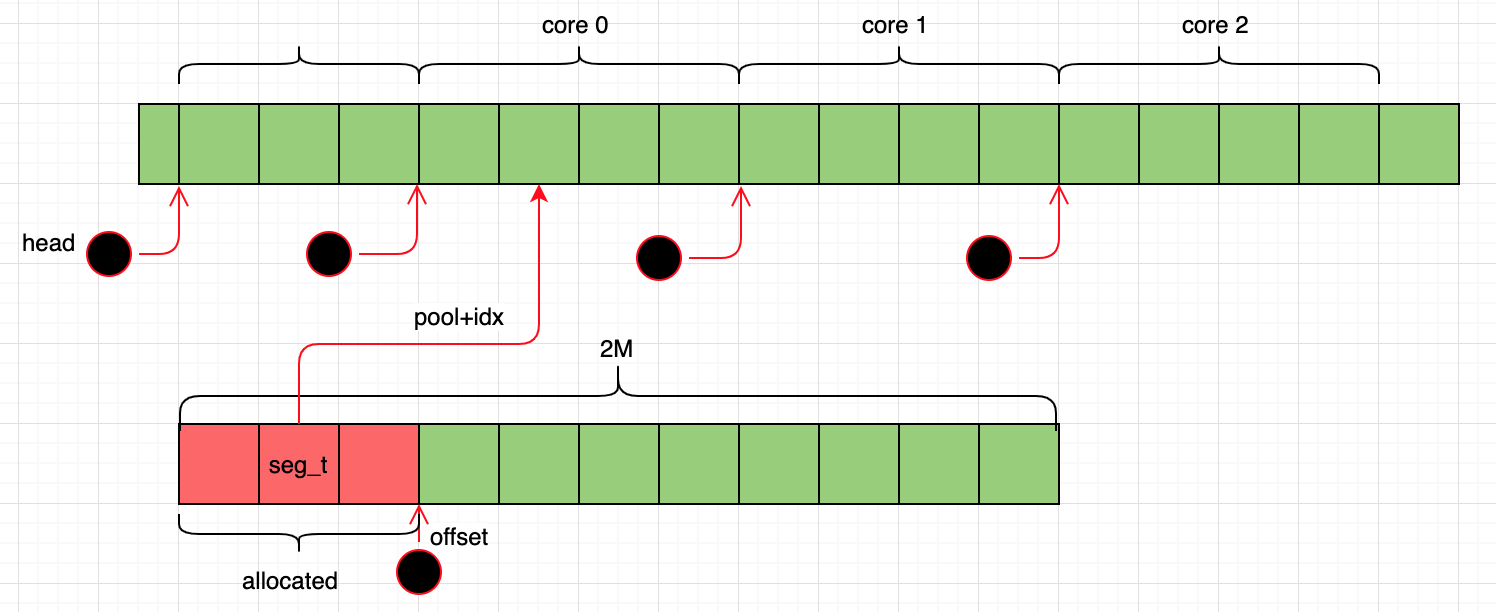
\includegraphics[width=10cm]{../imgs/buffer-t.png}
\end{center}

每个内存区域的\hl{第一个hugepage用来保存该区域的元数据信息},可供分配的是后面的hugepages。
在元数据信息中加上buddy,可用来支持buddy算法。

buffer的每个seg都包含有虚拟地址和物理地址。

\subsection{Memory Pool}

\begin{center}
    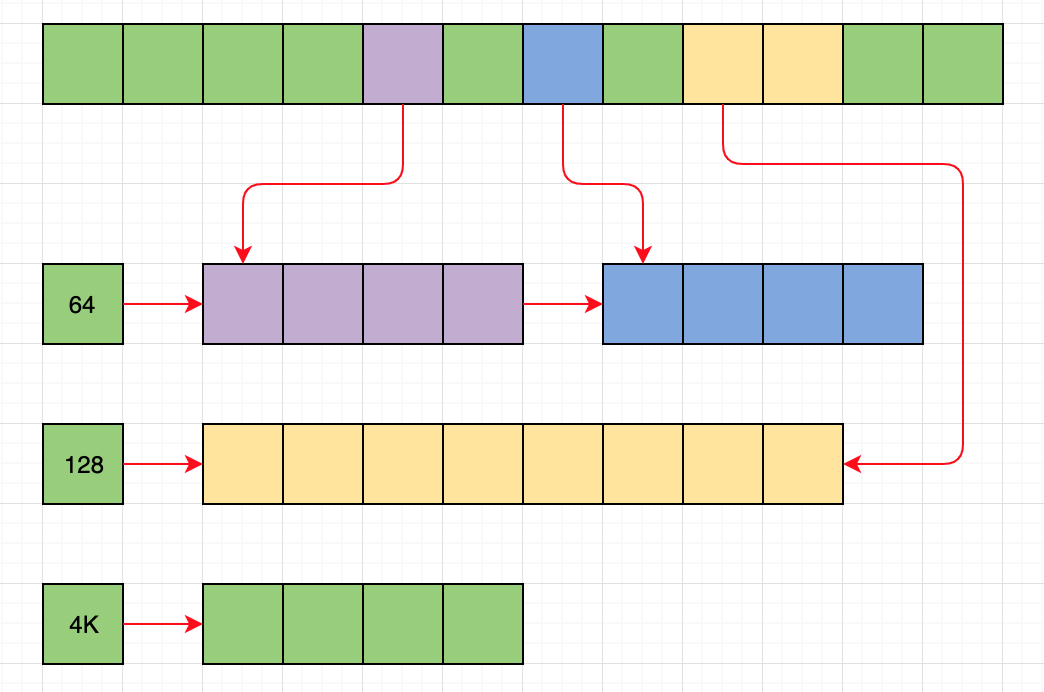
\includegraphics[width=10cm]{../imgs/memory-pool.png}
\end{center}

直接从hugepage申请内存,从hugepage申请一个hugepage,用于小对象。pool管理多个size的小对象队列。
根据要malloc的size,定位到队列。

free时按指针查找属于哪个hugepage。每个hugepge对应起始地址和结束地址以及所在队列的标识。
这样可以保留malloc和free的语法和语义。

hugepage层只需要提供分配单个hugepage的接口,一个队列可以由一个或多个hugepage构成。

或者,memory pool按4k进行组织,同样采用buddy算法。在其上实现ring等。

\hl{每layer都要动态化,包括增和减}。

\subsection{NVMe}

NVMe为什么需要物理地址?

direct io需要512对齐。

\subsection{RDMA}

每个连接$1024*512$内存。

\subsection{IO}

\begin{center}
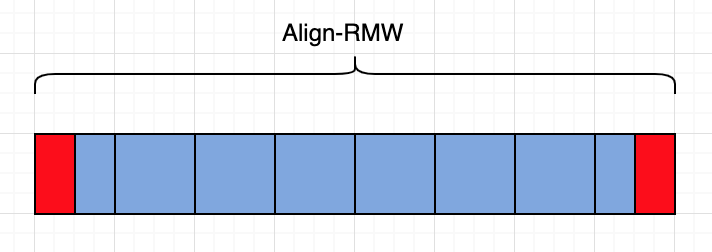
\includegraphics[width=10cm]{../imgs/io-align.png}
\end{center}

首尾页对齐

buffer\_t包含一个seg时,方便处理。如果有多个seg,是否需要分配连续的大块内存。

\hl{SPDK的大IO问题}:NVMe需要物理内存,并且一次io物理内存是连续的。
malloc的内存,不容易找到物理内存。
2M的hugepage虽然能获取虚拟地址连续的4M地址空间,但底层物理内存未必连续。
用1G的hugepage更容易管理。

GFM的机制是什么?barrier去解决RMW、chunk恢复等问题?

\chapter{作为一个操作系统}

\section{硬件}

硬件特性: 一台服务器有多个NUMA节点,每个NUMA节点包含多个core。
一个NUMA节点访问本地内存速度快、访问别的NUMA节点速度慢。
NUMA节点的访问特性对编程意味着什么?

\begin{enumbox}
\item 列出所有CPU/core
\item 如何把线程绑定到core上(设置处理器亲和性)
\item core线程维护TLS和私有memory allocator
\item core与memory存在什么样的关系,最终表现为访存latency
\end{enumbox}

\section{Scheduler}

从操作系统的角度去理解协程。协程也意味着执行的不连续性,与上下午切换。
协程有独立的调度器,负责从就绪队列里选出下一个要执行的任务。

站在scheduler的角度看,coroutine并无大的不同,只是实现了yield和resume方法。
通过任务队列进行调度,选出下一个要运行的协程。
协程是非抢占的,没有yield的话,在执行完后返回。

站在线程执行的角度看,scheduler和其它任务也无不同,看指令流顺序执行。
这是回到执行过程本质的观点。

\subsection{实现}

系统可以指定几个core,专门处理IO。每个core关联一个core thread,运行scheduler代码。

本质上,所谓的scheduler,就运行特定指令序列的操作系统线程,通过操作特定的数据结构和上下文切换,
模拟协程行为。

别的线程要与core thread通信,需要进行同步。core thread内部,不需要同步措施。

调度器和协程代码,交错执行。调度器切换到task,则执行task指令;
task让出控制权,或者返回,则执行调度器指令。

创建task,通过makecontext管理task要执行的过程,通过swapcontext在调度器和task之间切换上下文。

task的生灭过程,一个task的生命周期,状态变迁:FREE, RUNABLE/READY, RUNNING, SUSPEND, BACKTRACE。

BACKTRACE用于打印日志,扫描每一个task,检查task的存活时间。目前,不允许有特长时间的任务存在。
BACKTRACE是由调度器发起的。BACKTRACE不检查sleep状态的task。

每个task,有parent,从而构成task树。

目前维护有三个task队列(runable, reply\_local, reply\_remote),两个新的申请队列(wait\_task, request\_queue)。

task队列占用tasks槽位,总数受限,\hl{目前默认为1024个槽位}。

调度器支持优先级队列:引入不同于runable的队列,多队列之间分配时间片。

Actor编程模型,SEDA高并发架构。

\subsection{使用}

\subsubsection{接口}

\subsubsection{使用模式}

\subsubsection{FAQ}

\begin{compactenum}
\item schedule\_yield1 timeout。检查的是\hl{从yield到再次唤醒的时间,而不是任务的age,一个task可以多次yield/resume}
\item tasks槽位占满后,再加入的请求会放入wait list。task和wait list之间,可能形成相互依赖的deadlock。
\item schedule\_task\_get和schedule\_yield1必须配对使用
\end{compactenum}

\section{内存}

要解决的问题,一并发下的扩展性;二是碎片化。

通过buddy allocator解决外部碎片,通过slab allocator解决内部碎片。
在page allocator的基础上采用object pool模式。

\begin{enumbox}
\item page table
\item TLB
\item cache line
\item false share
\end{enumbox}

每个core线程拥有私有内存,但不应静态分配一个固定值,而是动态按需分配。
因为每个core线程所需内存量可能不均衡,出现总量够,而单个core内存不足的情况。

malloc返回的是虚拟地址,还没有分配物理地址。

预留、总量

优化项:
\begin{enumbox}
\item 减少代码体积
\item IO路径上的函数放入同一代码段
\item O3编译选项
\item inline
\item 去掉debug和info信息
\item variable\_t
\item lock table
\item hash table
\item replica\_srv\_get
\end{enumbox}

分析工具:
\begin{enumbox}
\item perf
\item lmbench
\end{enumbox}

\subsection{资源池模式}

一次从OS申请固定数量的hugepage,用buddy算法管理其alloc、free过程。
所谓buddy,就是管理一段连续内存单元,随着alloc、free的过程进行拆分与合并的规则。
最开始的时候,整个区域是连续的、每个节点跟踪记录所能分配的最大连续内存单元。

ring\_pool是固定大小的内存池,可以循环使用。

\subsection{Mem\_Cache}

两种分类
\begin{enumbox}
\item 分为两类:core线程私有与公共部分。
\item slab,分类,每类固定大小,可以自如伸缩。
\end{enumbox}

\subsection{Others}

\begin{enumbox}
\item jemalloc
\item tcmalloc
\item boost::pool
\end{enumbox}

\section{控制器}

目录和卷,都通过controller进行管理。目录controller的概念有待进一步完善。

每个控制器都可以看着一chunk树,其根节点对应chunk的副本位置列表,决定了控制器的位置:列表中第一副本所在节点。
在迁移控制器时,同样需要遵循该规则,所以需要先调整根chunk的chkinfo。

所有卷的操作都需要通过controller进行。客户端在访问一个卷时,第一步要找到该卷控制器的所在节点nid,
然后把nid作为参数传入后续调用中,如nid是客户端,则进程内;否则,发起rpc调用。
本地访问也可走rpc,可以利用rpc timeout等特性。

md\_map是控制器位置缓存,如可以在cache里找到,直接返回。如缓存不命中,则发起UDP广播。
每个lichd进程有独立线程监听端口:20915。检查cluster uuid,magic,crc等匹配后,尝试加载控制器,然后做出回应。
发起UDP广播的客户端收集各lichd进程的响应,如找到匹配的nid,可以直接退出该过程。

控制器加载过程:第一副本非本节点,返回EREMCHG。加载成功后,用vctl缓存管理起来,缓存项带引用计数和删除标志。
目前,采用lease机制保证vctl的唯一性。其必要性可进一步推演。
加载过程需要保证并发下的唯一性,如果有多个task发起加载过程,只有一个实际执行,别的进入等待队列。
加载完成后,唤醒等待队列里的任务。

\section{调度}

\section{I/O}

\subsection{Disk Allocator}

\subsection{Sqlite}

\subsection{FS}

\subsection{SPDK}

因为提交性能极高,不会block主线程,不需采用AIO。

\section{通信}

SCSI是节点与设备,节点与节点之间的通信协议。
SCSI over TCP/IP就是iSCSI,即SCSI/iSCSI/TCP协议栈,iSCSI over RDMA是iSER。

NVMe与SCSI是竞争协议,是演化方向。节点与设备:NVMe over PCIe。
节点之间则是NVMe over fabric(NVMf)。fabric与PCIe是不同的连接通道,泛指节点之间的通信链路。

\subsection{RPC}

封装底层不同链路,如TCP、或RDMA,提供统一的通信入口。

VM与target,可采用vhost方式,即IPC。

\subsection{RDMA}

一是initiator与target之间(SCSI或NVMe协议);二是各节点的corenet之间(什么协议?)。

\chapter{FAQ}

问题集:
\begin{enumbox}
\item /的位置信息
\item 当前分配的最大卷ID?
\end{enumbox}

P1: IOMeter测试,256K,Lich顺序和随机IO性能差别大

P2: lsv\_gc\_check断言失败

P3: Error Handling

\chapter{BUG}

\section{依赖性}

\begin{enumbox}
\item 线程存在依赖性,乱序退出产生core
\end{enumbox}

\section{writeback}

\verb|__writeback_flush__|


% \section{控制器}

目录和卷,都通过controller进行管理。目录controller的概念有待进一步完善。

每个控制器都可以看着一chunk树,其根节点对应chunk的副本位置列表,决定了控制器的位置:列表中第一副本所在节点。
在迁移控制器时,同样需要遵循该规则,所以需要先调整根chunk的chkinfo。

所有卷的操作都需要通过controller进行。客户端在访问一个卷时,第一步要找到该卷控制器的所在节点nid,
然后把nid作为参数传入后续调用中,如nid是客户端,则进程内;否则,发起rpc调用。
本地访问也可走rpc,可以利用rpc timeout等特性。

md\_map是控制器位置缓存,如可以在cache里找到,直接返回。如缓存不命中,则发起UDP广播。
每个lichd进程有独立线程监听端口:20915。检查cluster uuid,magic,crc等匹配后,尝试加载控制器,然后做出回应。
发起UDP广播的客户端收集各lichd进程的响应,如找到匹配的nid,可以直接退出该过程。

控制器加载过程:第一副本非本节点,返回EREMCHG。加载成功后,用vctl缓存管理起来,缓存项带引用计数和删除标志。
目前,采用lease机制保证vctl的唯一性。其必要性可进一步推演。
加载过程需要保证并发下的唯一性,如果有多个task发起加载过程,只有一个实际执行,别的进入等待队列。加载完成后,唤醒等待队列里的任务。

% \chapter{Scheduler}

从操作系统的角度去理解协程。协程也意味着执行的不连续性,与上下午切换。
协程有独立的调度器,负责从就绪队列里选出下一个要执行的任务。

\section{实现}

系统可以指定几个core,专门处理IO。每个core关联一个core thread,运行scheduler代码。

本质上,所谓的scheduler,就运行特定指令序列的操作系统线程,通过操作特定的数据结构和上下文切换,
模拟协程行为。

别的线程要与core thread通信,需要进行同步。core thread内部,不需要同步措施。

调度器和协程代码,交错执行。调度器切换到task,则执行task指令;
task让出控制权,或者返回,则执行调度器指令。

创建task,通过makecontext管理task要执行的过程,通过swapcontext在调度器和task之间切换上下文。

task的生灭过程,一个task的生命周期,状态变迁:FREE, RUNABLE/READY, RUNNING, SUSPEND, BACKTRACE。

BACKTRACE用于打印日志,扫描每一个task,检查task的存活时间。目前,不允许有特长时间的任务存在。
BACKTRACE是由调度器发起的。BACKTRACE不检查sleep状态的task。

每个task,有parent,从而构成task树。

目前维护有三个task队列(runable, reply\_local, reply\_remote),两个新的申请队列(wait\_task, request\_queue)。

task队列占用tasks槽位,总数受限,\hl{目前默认为1024个槽位}。

调度器支持优先级队列:引入不同于runable的队列,多队列之间分配时间片。

Actor编程模型,SEDA高并发架构。

\section{使用}

\subsection{接口}

\subsection{使用模式}

\subsection{FAQ}

\begin{compactenum}
\item schedule\_yield1 timeout。检查的是\hl{从yield到再次唤醒的时间,而不是任务的age,一个task可以多次yield/resume}
\item tasks槽位占满后,再加入的请求会放入wait list。task和wait list之间,可能形成相互依赖的deadlock。
\item schedule\_task\_get和schedule\_yield1必须配对使用
\end{compactenum}


\part{LichMaster}
\chapter{Lich Master}

\section{MM}

\subsection{问题}

\begin{enumbox}
\item 简单接口
\item 便于调试
\item 并发性能
\item 内外碎片
\item 动态化
\item RDMA内存
\item replica\_srv\_init不能利用core内存,模块依赖性
\item Hash局部性不好,不利于CPU高速缓存
\end{enumbox}

\subsection{现状}

源文件:
\begin{enumbox}
\item ylib/lib/mem.c
\item ylib/lib/mem\_hugepage.c
\item ylib/lib/mem\_cache.c
\item ylib/lib/mem\_pool.c
\item ylib/lib/buddy.c
\item ylib/lib/buffer.c
\end{enumbox}

两级内存管理

分为core内外两种情况:core使用私有内存。

先生成hugepage,并置0。malloc后得到虚拟地址空间,把hugepage依次mmap到该虚拟地址空间。

hugepage与numa物理内存的关系是怎么样的?什么时候建立起来的?

底层hugepage不一定要用buddy,并且应可动态扩展。
然后是pool层,可动态扩展,用buddy管理每个hugepage。
其上是对象层slot,用于分配应用对象,用大小不等的多个队列管理。

RDMA需要注册内存,目前是把整个core内存一次性注册了。
每个core都调用注册函数?

\section{RDMA}

\begin{enumbox}
\item RDMA的编程模型?
\item RDMA的连接管理过程?
\item RDMA的内存使用方式有什么不同?
\item iSCSI/iSER conn是如何关联起来的?
\item 更好的抽象?
\end{enumbox}

RDMA是与TCP并列的一种网络传输方式,需要特定硬件支持,包括RDMA的NIC与交换机。
网络设备不同于存储设备,RDMA可以carry任意网络流量,包括iSCSI/iSER,自定义协议(corenet)等。

ibverbs API屏蔽了链路层的不同,可以用一套API同时支持IB,RoCE、iWARP等。

\subsection{ibverbs}

分为几个层次:node、core/dev、conn、event。

每个设备对应rdma\_info\_t结构,有ibv\_context属性,是唯一的key。
rdma\_cm\_id具有该属性。

\begin{itembox}
\item pd
\item cq (被所有连接共享)
\item mr  (shared)
\end{itembox}

深刻理解一个RDMA连接管理的过程,建立连接的每个阶段需要做哪些工作?

每个RDMA连接,qp关联到cq上。cq\_poll。iov\_mr

qp支持ibv\_post\_recv操作,peer的send操作会消耗这些buffer,
在与远端建立之后,就应注册相关buffer,建立必要的关系,特别是指定wr\_id属性,并post,然后等待接受请求。

在ibv\_cq\_poll之后,得到的ibv\_wc里,包含所需上下午信息(post之前建立的关系,初始化task时)。
可以直接从buffer里recv到的数据。

RDMA是异步通信机制。

\subsection{MM}

RDMA通信包括两类:msg与数据读写,所需内存都需要register。

向RNIC注册内存

\subsection{建立连接}

采用epoll机制

\subsection{通信}

采用ibv\_cq\_poll机制

\subsection{协议-iSER}

iSCSI over RDMA

iSCSI分多阶段,包括Login、Full Feature等。

\subsection{协议-NVMf}

NVMe over Fabric

\section{NVMe}

\subsection{SPDK}

\section{Performance}

\subsection{Hash}

\begin{enumbox}
\item Lock table
\item Replica srv
\end{enumbox}


\part{生态系统}

\chapter{LVM}

clvm

\chapter{Tgt}

Tgt

\chapter{CEPH}

\chapter{Nutanix}

zookeeper

cassandra

数据和I/O本地化

ROW快照和克隆

DR

%\include{sheepdog}
%\include{openvstorage}
%\include{VSAN}

\part{理论基础}

\chapter{Sites}

Projects
\begin{myeasylist}{itemize}
& \url{https://spdk.io/}
& \url{https://nvmexpress.org/resources/specifications/}
& \url{https://www.techrepublic.com/}
& \url{https://www.itcentralstation.com/products/comparisons/e8-storage_vs_pure-storage-flasharray}
& \url{https://insidehpc.com/2019/04/thinkparq-brings-beegfs-to-e8-storage/}
\end{myeasylist}

Linux
\begin{myeasylist}{itemize}
& \url{http://ifeve.com/memory-barriers-or-fences/}
& \url{https://etcd.io/docs/v3.3.12/learning/api/#revisions}
& \url{https://jepsen.io/consistency}
& \url{http://www.tpc.org/tpcc/}
\end{myeasylist}

Tools
\begin{myeasylist}{itemize}
& \url{https://www.mindtools.com/}
& \url{https://www.isixsigma.com/dictionary/}
& \url{http://astyle.sourceforge.net/}
\end{myeasylist}

Network
\begin{myeasylist}{itemize}
& \url{https://docs.mellanox.com/pages/viewpage.action?pageId=12013422#RDMAoverConvergedEthernet(RoCE)-AssociatingInfiniBandPortstoEthernetPorts}
& \url{https://community.mellanox.com/s/article/howto-set-the-default-roce-mode-when-using-rdma-cm}
& \url{https://www.cnblogs.com/burningTheStar/p/8565612.html}
\end{myeasylist}

Oracle
\begin{myeasylist}{itemize}
& \url{https://www.oracle.com/database/technologies/rac/asm.html}
\end{myeasylist}

News
\begin{myeasylist}{itemize}
& \url{https://chuansongme.com/account/huangliang_storage?start=0}
& \url{http://stor-age.zhiding.cn/}
\end{myeasylist}

SPDK
\begin{myeasylist}{itemize}
& \url{https://www.sdnlab.com/23178.html}
\end{myeasylist}

\chapter{算法}

\section{排序算法}

\subsection{Insertion Sort}

\subsection{Shell Sort}

\subsection{Select Sort}

\subsection{Heap Sort}

\subsection{Bubble Sort}

\subsection{Quick Sort}

\subsection{Merge Sort}

归并,多路归并,外排序

\subsection{Counting Sort}

\subsection{Bucket Sort}

\subsection{Radix Sort}

\section{查找算法}

\subsection{二分查找}

\subsection{TOP N}

\chapter{数据结构}

array和list是存储结构,大部分ADT都依赖于此。

\section{Bit}

\subsection{BloomFilter}

\section{String}

\section{Array}

\section{List}

\subsection{SkipList}

\section{Stack}

\section{Queue}

scheduler

\section{Hash}

hash函数,hash局部性不佳(影响CPU高速缓存性能),大的hash表最好分组,极限情况是radix tree。
Linux Page Cache采用了radix tree,而不是hash。

\section{Heap}

TopN,多路归并,从TopN中再选出TopN

\section{Tree}

\subsection{Binary Search Tree}

\subsection{B and B+ Tree}

\subsection{Red Black Tree}

\subsection{Radix Tree}

tier

\subsection{Huffman Code}

\section{Graph}

\section{Bit}

\subsection{Bmap}

\subsection{Bmap Index}

\subsection{BloomFilter}

是一个查找结构。

\section{String}

\begin{enumbox}
\item c: char array
\item c++: string class
\item Java: StringBuilder
\item re
\end{enumbox}

\chapter{编程语言}

\section{C++}

\chapter{服务端软件架构}

从节点到集群,从本地到全局

平衡利用各种资源。

\section{引言:C1000K问题}

\section{调度}

\subsection{Actor}

controller类似actor概念。

non-blocking IO。

带队列的线程是一个强大的结构,即有执行单元,又有调度单元。一些复杂的任务,比如恢复过程中的并行执行,就最好组织成带队列的线程池。
至于队列是线程私有,还是公共队列,是一个需要进一步探讨的问题。

再比如,协程调度本质上也是一个带队列的线程,队列不止一个,可以组合成相对强大的调度模型。

\subsection{CSP}

显式channel

\subsection{SEDA}

actor + pipeline,多个actor构成SEDA架构。

\section{Memory}

内存分配也是syscall,经过glib包装后,依然不能满足高性能要求。

\begin{enumbox}
\item hugepage
\item 两层allocator,解决内外碎片问题;
\item buffer\_t解决zero-copy。
\item core thread拥有私有内存,解决共享/竞争问题。
\end{enumbox}

\section{EIT}

\begin{itemize}
    \item journalling
    \item update many, commit one
    \item double check
    \item double/multi buffer
    \item half sync, half async
\end{itemize}

\chapter{性能优化}

\section{高性能架构}

从软件与硬件多个层面去梳理整个问题。

首先看资源、架构、算法,以及评估标准,或指标,接着进行设计方法、模式的研究。

新硬件:3+1都在演化。内存、外存的界限、波谱趋于平滑过渡。

新架构:使用硬件资源的方式也在发生变化,从操作系统、编程语言到应用层都是如此。
Intel SPDK/DPDK是个巨大的突破。
tgt项目有iSER,NVMf的实现。
bcache、Flashcache解决io路径的特定问题。

定制memory allocator是一个新认知。

SCSI的演化:

怎么设计出具有竞争力的系统?

\section{学习资料}

阅读yufeng,何登成blog。

性能杀手
\begin{enumbox}
\item context switch 
\item Lock 
\item memory malloc
\item data copy
\item System call 
\item false share
\end{enumbox}

理论
\begin{enumbox}
\item USE方法
\item 算法分析
\item 排队论
\end{enumbox}

Tool
\begin{enumbox}
\item top
\item iotop
\item slabtop
\item free
\item vmstat
\item iostat
\item dstat
\item pidstat
\item *
\item tcpdump
\item netstat
\item mpstat
\item tcprstat
\item nicstat
\item *
\item strace
\item blktrace
\item stap
\item perf
\item oprofile
\item stap
\item lmbench
\end{enumbox}


\chapter{计算机体系结构}

组成原理与体系结构,研究内容相当。

\section{结构}

三部分:CPU,存储器,I/O设备。PCIe和NUMA都采用分布式架构,PCIe是串行点对点,
NUMA分远和近,访问远程CPU慢。可以称为分布式共享内存。

二进制

进制之间的转换
\begin{enumbox}
\item 整数(除2取余)
\item 负数(取反加1)
\item 小数(乘2取整)
\item 浮点数采用科学计数法,分单精度与双精度
\item 高位是符号位
\item 表示范围不变,坐标平移
\end{enumbox}

字节顺序:32bit机器上字长是4B,64bit机器上字长是8B。
一个字的字节采用由左到右编码,或从右到左编码。
big-endian表示尾端在高位,little-endian表示尾端在低位。

\section{执行}

一颗CPU的执行可以看着一维的指令流,由顺序和跳转指令,由调度程序模拟多任务的假象。
并发执行需要进行同步,以避免引起的问题,保证数据的一致性和安全性、执行结果的准确性。

基于lock的同步,可能会引起死锁或饥饿现象,须加以避免、检测。

进程的五状态模型,进程调度算法

流水线并行示意图

协同过程,又称协程,控制权转移,可以不从函数开始处执行。

指令执行,需要在寄存器与主存间同步数据。
主存的值,须加载到寄存器。\hl{CPU指令能直接访问主存内容吗?}

物理内存大小固定,需要虚拟化,供多个进程使用。进程的地址空间彼此隔离。
由页表和TLB执行逻辑地址到物理地址的映射。
\hl{物理地址如何管理?分配和回收是否需要free list或bitmap一样的索引结构?}

Hugepage可以减小页表的大小,加快检索性能。

进程空间分用户空间和kernel空间。用户进程空间分段管理:text,data,bss,heap,stack。

进程-进程空间-内存-I/O是核心概念,是理解的主要节点。物理内存不足时,可以借用部分磁盘swap空间,
但这种情况会引起频繁的swap in/out,造成性能抖动。

程序的执行过程:汇编、链接、加载。加载后生成一进程,参与调度。

\chapter{Linux Kernel}

操千曲而后晓声,观千剑而后知器。

\chapter{操作系统}

资源管理,架起硬件和上层应用之间的桥梁。资源的3+1模型:cpu、memory、disk and network。

\section{CPU}

从单核cpu说起,多核cpu引入了哪些关键问题?

进程、线程、协程调度

通信和同步

经典问题:
\begin{compactenum}
\item 生产者-消费者问题
\item 读者-写者问题
\item 哲学家就餐问题
\end{compactenum}

\section{Memory}

\section{IO和文件系统}

\section{分布式系统}

% \include{basic/compiler}
\chapter{文件系统}

\section{Fuse}

在mount的时候,向kernel注册handler。

\section{GlusterFS}

\chapter{数据库系统}

从操作系统开始到数据库管理系统,对并发现象的讨论,上升到新的高度。
硬件提供了基础原子指令,利用这些原子指令封装成并发原语,
进一步去实现事物的ACID要求。

计算模型:事务的页模型和对象模型。对象模型是页模型的一个推广,对象模型的叶子节点是页,构成一棵树。

没有什么比好的理论更有用。透过页模型可以推演出很多重要结论。
并发控制算法、事务恢复、分布式提交是由简单到复杂的推演路径。
前两个可以在单节点环境下讨论,然后提升到分布式环境下,引出分布式提交的概念。

答案并非唯一,多种答案之间权衡利弊得失。

\section{并发问题}

并发访问共享对象,竞态条件

\begin{enumbox}
\item 过程是否发生了yield,不连续执行?
\item 临界区有哪些共享对象?
\item 冲突操作
\item 如果有多个并发任务重入该过程,会造成什么问题?
\item 加锁的粒度如何,太大,或太小?
\item 乱序?
\item 有无lock free,wait free方案?
\end{enumbox}

\section{事务管理}

事务模型、详解ACID。

\subsection{隔离等级}

\section{可串行化理论}

单站点的可串行化,单副本可串行化(RSM)

冲突操作:优先图的节点是事务,节点之间的边是冲突操作对。无环时是可串行调度。

\section{2PL}

2PL可以保障事务串行化。注意加锁的顺序和解锁的顺序。

索引结构上的加锁规则

lock-free queue:并非无锁,而是小锁。

\section{并发设计模式}

意向锁?

范围锁?

\begin{compactitem}
    \item double check
    \item fork and join
    \item pipeline
    \item half sync, half async
\end{compactitem}

\section{故障恢复}

基于日志的恢复

REDO

UNDO

\chapter{Big Data}


\chapter{并发}

编程模型:多线程和事件驱动。多线程访问共享内存,需要同步机制。锁会形成死锁。
事件驱动有主循环,不能调用block操作,另外涉及如何动态扩展到多核多CPU的环境。

actor编程模型,SEDA是一个特殊的actor架构。

进程及其通信是基础模型。执行的代换模型与环境模型,事务的页模型与对象模型,
由简单模型推导关键结论。

并行有两种:竞争并行与协作并行。

\section{PCAM设计方法学}

\begin{enumbox}
\item 划分 数据划分、任务划分
\item 通信 任务之间的数据交换
\item 聚合 合并任务,以提升性能
\item 映射 任务调度,并符合负载均衡
\end{enumbox}

\subsection{Example:volume}

volume是一个自然划分,把volume映射到一个core thread上。
问题是这样做的话,粒度过大,无法有效进行负载均衡,受限于单core最大处理能力。

如果一个subvol映射到一个core thread,粒度合适。但需要引入复杂的控制机制。
最好是映射到一个节点的多个core上。

以上分析过程用到了完整的PCAM方法。

\subsection{Example:recovery}

\subsection{Example:rmvol}

无需通过controller去做这些事情,可以直接利用db信息。

\subsection{Example:rollback}

\subsection{Example:flatten}

\section{同步原语}

同步原语组成层次结构。并发原语,层层还原,层层构建

从OS到DB,对并发的讨论在深化,事务要求ACID,且访问特定的索引结构。
另外还有持久化的要求,原子写变得更困难,引入日志。

本质上是序的问题,锁内在地实现了一种序。
逻辑时钟、paxos、raft中,序起到了至关重要的作用。

\chapter{分布式系统}

Lich涉及许多底层理论和系统,包括并行计算和分布式系统,操作系统,文件系统,数据库系统,网络,还包括相应的底层硬件架构。
需要对数据结构和算法,有良好基础。所以,对基本问题和理论,要有清晰和深入的掌握,才能“运用之妙,存乎一心”。

存储中一些重要的问题,可以借助AI的力量去解决。智能存储,不仅仅是口号,更是技术进步的必要趋势。

按道法术器组织结构,写成大文章。

常用优化原则:
\begin{itemize}
    \item 局部性
    \item 并行
    \item 聚合,批处理
    \item 延迟
\end{itemize}

\section{2PC}

\section{Paxos}
\section{RAFT}



\chapter{Tools}

\section{debug}

trace msgid来跟踪消息流。

\section{cmake}

\begin{center}
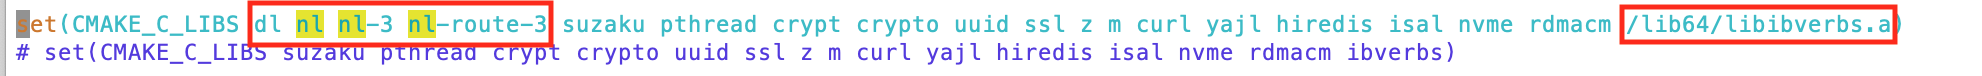
\includegraphics[width=10cm]{../imgs/cmake-link-static.png}
\end{center}

生成静态库
\begin{myeasylist}{itemize}
& SHARED  -> STATIC
& LIBRARY -> ARCHIVE
\end{myeasylist}

\section{gdb}

\begin{myeasylist}{itemize}
& ~/.gdbinit
& info registers
& info sharedlibrary
& gdb -p
\end{myeasylist}

gdb -p发现了mbuffer\_writefile进入死循环,原因是count==0。

猜想是重入了一个锁。

\section{wireshark}

\chapter{FlowChart}

% 流程图定义基本形状
\tikzstyle{startstop} = [rectangle, rounded corners, minimum width=3cm, minimum height=1cm,text centered, draw=black, fill=red!30]
\tikzstyle{io} = [trapezium, trapezium left angle=70, trapezium right angle=110, minimum width=3cm, minimum height=1cm, text centered, draw=black, fill=blue!30]
\tikzstyle{process} = [rectangle, minimum width=3cm, minimum height=1cm, text centered, draw=black, fill=orange!30]
\tikzstyle{decision} = [diamond, minimum width=3cm, minimum height=1cm, text centered, draw=black, fill=green!30]
\tikzstyle{arrow} = [thick,->,>=stealth]

\begin{tikzpicture}[node distance=2cm]
%定义流程图具体形状
\node (start) [startstop] {Start};
\node (in1) [io, below of=start] {Input};
\node (pro1) [process, below of=in1] {Process 1};
\node (dec1) [decision, below of=pro1, yshift=-0.5cm] {Decision 1};
\node (pro2a) [process, below of=dec1, yshift=-0.5cm] {Process 2a};
\node (pro2b) [process, right of=dec1, xshift=2cm] {Process 2b};
\node (out1) [io, below of=pro2a] {Output};
\node (stop) [startstop, below of=out1] {Stop};

%连接具体形状
\draw [arrow](start) -- (in1);
\draw [arrow](in1) -- (pro1);
\draw [arrow](pro1) -- (dec1);
\draw [arrow](dec1) -- (pro2a);
\draw [arrow](dec1) -- (pro2b);
\draw [arrow](dec1) -- node[anchor=east] {yes} (pro2a);
\draw [arrow](dec1) -- node[anchor=south] {no} (pro2b);
\draw [arrow](pro2b) |- (pro1);
\draw [arrow](pro2a) -- (out1);
\draw [arrow](out1) -- (stop);
\end{tikzpicture}

%作者:红伞菌
%链接:https://www.zhihu.com/question/20854046/answer/16400909
%来源:知乎
%著作权归作者所有。商业转载请联系作者获得授权,非商业转载请注明出处。
%作者:红伞菌
%链接:https://www.zhihu.com/question/20854046/answer/16400909
%来源:知乎
%著作权归作者所有。商业转载请联系作者获得授权,非商业转载请注明出处。

% Defines a `datastore' shape for use in DFDs.  This inherits from a
% rectangle and only draws two horizontal lines.
\makeatletter
\pgfdeclareshape{datastore}{
  \inheritsavedanchors[from=rectangle]
  \inheritanchorborder[from=rectangle]
  \inheritanchor[from=rectangle]{center}
  \inheritanchor[from=rectangle]{base}
  \inheritanchor[from=rectangle]{north}
  \inheritanchor[from=rectangle]{north east}
  \inheritanchor[from=rectangle]{east}
  \inheritanchor[from=rectangle]{south east}
  \inheritanchor[from=rectangle]{south}
  \inheritanchor[from=rectangle]{south west}
  \inheritanchor[from=rectangle]{west}
  \inheritanchor[from=rectangle]{north west}
  \backgroundpath{
    %  store lower right in xa/ya and upper right in xb/yb
    \southwest \pgf@xa=\pgf@x \pgf@ya=\pgf@y
    \northeast \pgf@xb=\pgf@x \pgf@yb=\pgf@y
    \pgfpathmoveto{\pgfpoint{\pgf@xa}{\pgf@ya}}
    \pgfpathlineto{\pgfpoint{\pgf@xb}{\pgf@ya}}
    \pgfpathmoveto{\pgfpoint{\pgf@xa}{\pgf@yb}}
    \pgfpathlineto{\pgfpoint{\pgf@xb}{\pgf@yb}}
 }
}
\makeatother
\begin{center}
\begin{tikzpicture}[
  font=\sffamily,
  every matrix/.style={ampersand replacement=\&,column sep=2cm,row sep=2cm},
  source/.style={draw,thick,rounded corners,fill=yellow!20,inner sep=.3cm},
  process/.style={draw,thick,circle,fill=blue!20},
  sink/.style={source,fill=green!20},
  datastore/.style={draw,very thick,shape=datastore,inner sep=.3cm},
  dots/.style={gray,scale=2},
  to/.style={->,>=stealth',shorten >=1pt,semithick,font=\sffamily\footnotesize},
  every node/.style={align=center}]

  % Position the nodes using a matrix layout
  \matrix{
    \node[source] (hisparcbox) {electronics};
      \& \node[process] (daq) {DAQ}; \& \\

    \& \node[datastore] (buffer) {buffer}; \& \\

    \node[datastore] (storage) {storage};
      \& \node[process] (monitor) {monitor};
      \& \node[sink] (datastore) {datastore}; \\
  };

  % Draw the arrows between the nodes and label them.
  \draw[to] (hisparcbox) -- node[midway,above] {raw events}
      node[midway,below] {level 0} (daq);
  \draw[to] (daq) -- node[midway,right] {raw event data\\level 1} (buffer);
  \draw[to] (buffer) --
      node[midway,right] {raw event data\\level 1} (monitor);
  \draw[to] (monitor) to[bend right=50] node[midway,above] {events}
      node[midway,below] {level 1} (storage);
  \draw[to] (storage) to[bend right=50] node[midway,above] {events}
      node[midway,below] {level 1} (monitor);
  \draw[to] (monitor) -- node[midway,above] {events}
      node[midway,below] {level 1} (datastore);
\end{tikzpicture}
\end{center}

\begin{figure}[htb]
\centering
%定义形状样式
\tikzstyle{startstop} = [rectangle, rounded corners, minimum width = 3cm, minimum height = 0.7cm, text centered, draw = black]
\tikzstyle{startstop2} = [rectangle, rounded corners, minimum width = 13cm, minimum height = 0.7cm, text centered, draw = black]
\tikzstyle{io} = [trapezium, trapezium left angle = 30, trapezium right angle = 150, minimum width = 3cm, text centered, draw = black, fill = white]
\tikzstyle{io2} = [trapezium, trapezium left angle = 30, trapezium right angle = 150, minimum width = 2.5cm, draw = black, fill = white]
\tikzstyle{io3} = [trapezium, trapezium left angle = 30, trapezium right angle = 150, minimum width = 2cm, draw = black, fill = white]
\tikzstyle{process} = [rectangle, minimum width = 3cm, minimum height = 1cm, text centered, draw = black]
\tikzstyle{decision} = [diamond, minimum width = 3cm, minimum height = 1cm, text centered, draw = black]
\tikzstyle{arrow} = [thick, -, >= stealth]
\tikzstyle{arrow2} = [thick, ->, >= stealth]

\begin{tikzpicture}[node distance = 1.5cm]
% 定义流程图具体形状
\coordinate[label = left:{\small 输入图像}](A) at(-1.5, 0);
\node(in1) [io] {};
\node(pro1) [startstop, below of = in1] {\small 线性滤波};

\node(in2 - 2)[io3, below of = pro1, yshift = -0.6cm]{};
\node(in3 - 2)[io3, left of = in2 - 2, xshift = -2.5cm]{};
\node(in4 - 2)[io3, right of = in2 - 2, xshift = 2.5cm]{};

\node(in2 - 1)[io2, below of = pro1, yshift = -0.3cm]{};
\node(in3 - 1)[io2, left of = in2 - 1, xshift = -2.5cm]{};
\node(in4 - 1)[io2, right of = in2 - 1, xshift = 2.5cm]{};

\node(in2) [io, below of = pro1] {\small 颜色};
\node(in3)[io, left of = in2, xshift = -2.5cm]{\small 亮度};
\node(in4)[io, right of = in2, xshift = 2.5cm]{\small 方向};

\node(in5)[startstop2, below of = in2 - 2]{\small Center - Surround差异计算及归一化};

\node(in6 - 2)[io3, below of = in5, yshift = -0.6cm]{};
\node(in7 - 2)[io3, left of = in6 - 2, xshift = -2.5cm]{};
\node(in8 - 2)[io3, right of = in6 - 2, xshift = 2.5cm]{};

\node(in6 - 1)[io2, below of = in5, yshift = -0.3cm]{};
\node(in7 - 1)[io2, left of = in6 - 1, xshift = -2.5cm]{};
\node(in8 - 1)[io2, right of = in6 - 1, xshift = 2.5cm]{};

\node(in6) [io, below of = in5] {};
\node(in7)[io, left of = in6, xshift = -2.5cm]{};
\node(in8)[io, right of = in6, xshift = 2.5cm]{};

\coordinate[label = left:{\small 特征图}](B) at(-1, -6.2);
\coordinate[label = left:{\small (12张)}](C) at(-1.5, -7.5);
\coordinate[label = left:{\small (6张)}](D) at(2.7, -7.5);
\coordinate[label = left:{\small (24张)}](E) at(6.7, -7.5);

\node(in9)[startstop2, below of = in6 - 2]{ \small 跨尺度合并及归一化 };

\node(in10) [io, below of = in9] {};
\node(in11)[io, left of = in10, xshift = -2.5cm]{};
\node(in12)[io, right of = in10, xshift = 2.5cm]{};

\coordinate[label = left:{\small 醒目图}](F) at(-1, -9.5);
\node(in13) [startstop, below of = in10] {\small 线性组合};
\node(in14) [io, below of = in13] {};
\coordinate[label = left:{\small 显著图}](G) at(-1, -13);

\node(in15) [startstop, below of = in14] {\small 赢者取全};
\coordinate[label = left:{\small 显著位置}]() at(1, -16.1);
\coordinate[label = left:{\small 反馈抑制}]() at(4.5, -14.7);

%连线
\draw[arrow](pro1) -- (in1);
\draw[arrow](pro1) -- (in2);
\draw[arrow](pro1) -- (in3);
\draw[arrow](pro1) -- (in4);
\draw[arrow](0, -4.75) -- (in2 - 2);
\draw[arrow](-4, -4.75) -- (in3 - 2);
\draw[arrow](4, -4.75) -- (in4 - 2);
\draw[arrow](0, -5.45) -- (in6);
\draw[arrow](-4, -5.45) -- (in7);
\draw[arrow](4, -5.45) -- (in8);
\draw[arrow](0, -8.35) -- (in6 - 2);
\draw[arrow](-4, -8.35) -- (in7 - 2);
\draw[arrow](4, -8.35) -- (in8 - 2);
\draw[arrow](0, -9.05) -- (in10);
\draw[arrow](-4, -9.05) -- (in11);
\draw[arrow](4, -9.05) -- (in12);
\draw[arrow](in13) -- (in10);
\draw[arrow](in13) -- (in11);
\draw[arrow](in13) -- (in12);
\draw[arrow](in13) -- (in14);
\draw[arrow](in14) -- (in15);
\draw[arrow](in15) -- (0, -15.8);
\draw[arrow](0, -15.4) -- (2.5, -15.4);
\draw[arrow](2.5, -14) -- (2.5, -15.4);
\draw[arrow2](2.5, -14) -- (0, -14);
\end{tikzpicture}
\caption{IT算法流程\cite{Itti}}
\end{figure}

% 设置颜色代号
\colorlet{lcfree}{green}
\colorlet{lcnorm}{blue}
\colorlet{lccong}{red}
% -------------------------------------------------
% 设置调试标志层
\pgfdeclarelayer{marx}
\pgfsetlayers{main,marx}
% 标记坐标点的宏定义。交换下面两个定义关闭。
\providecommand{\cmark}[2][]{%
  \begin{pgfonlayer}{marx}
    \node [nmark] at (c#2#1) {#2};
  \end{pgfonlayer}{marx}
  } 
\providecommand{\cmark}[2][]{\relax} 
% -------------------------------------------------
% 开始绘图
\begin{figure}[h]
\centering
\scalebox{.8}{                  %设置缩放	
\begin{tikzpicture}[
    >=triangle 60,              % 箭头的形状
    start chain=going below,    % 从上往下的流程
    node distance=6mm and 60mm, % 全局间距设置
    every join/.style={norm},   % 连接线的默认设置
    ]
% ------------------------------------------------- 
% 节点的样式定义 
% <on chain> 和 <on grid> 可以减少手动调整节点位置的麻烦
\tikzset{
  base/.style={draw, on chain, on grid, align=center, minimum height=4ex},
  proc/.style={base, rectangle, text width=8em},
  test/.style={base, diamond, aspect=2, text width=5em},
  term/.style={proc, rounded corners},
  % coord 用来表示连接线的转折点
  coord/.style={coordinate, on chain, on grid, node distance=6mm and 25mm},
  % nmark 用来表示调试标志
  nmark/.style={draw, cyan, circle, font={\sffamily\bfseries}},
  % -------------------------------------------------
  % 不同的连接线样式
  norm/.style={->, draw, lcnorm},
  free/.style={->, draw, lcfree},
  cong/.style={->, draw, lccong},
  it/.style={font={\small\itshape}}
}
% -------------------------------------------------
% 先放节点
\node [term, densely dotted,fill=lccong!25, it] (p0) {输入};
% 用 join 表示和上一个节点相连 
\node [proc, join]	{使用非线性最小二乘法得到 $X_0$};
\node [proc, join]	{记录 $X=X_0, f=f(X_0)$};
\node [test, join] (t1)	{$T>T_E$?};
\node [proc] (p1)		{$step=0$};
\node [test, join] (t2)	{$step<count$?};
\node [proc] (p2)		{得到新状态$P_N=P+scale\times rand$,计算目标函数差$\Delta f$};
\node [test, join] (t3)	{$F_{Accept}<rand$?};
\node [proc] (p3)		{记录新状态 $X=X_N,f=f(X_N)$};

\node [proc, left=of t1] (p4)	{$T=T\times a,scale=scale\times b$};
\node [term, densely dotted, right=of t1,fill=lcfree!25](p5)	{输出};
\node [proc, right=of t3](p6)	{$step++$};

\node [coord, left=of t2] (c1)  {}; 
\node [coord, right=of t2] (c2)  {}; 
\node [coord, right=of p3] (c3)  {}; 
%先画南北方向的连接线,先画线再画两端的标志和箭头
\path (t1.south) to node [near start, xshift=1em] {$y$} (p1);
  \draw [*->,lcnorm] (t1.south) -- (p1);
\path (t2.south) to node [near start, xshift=1em] {$y$} (p2);
  \draw [*->,lcnorm] (t2.south) -- (p2);
\path (t3.south) to node [near start, xshift=1em] {$y$} (p3);
  \draw [*->,lcnorm] (t3.south) -- (p3);
%接着画东西方向的连接线,方法同上
\path (t1.east) to node [near start, yshift=1em]  {$n$}(p5);
  \draw [o->,lcnorm] (t1.east) -- (p5);
  \draw [->,lcnorm] (p4.east) -- (t1);
\path (t3.east) to node [near start, yshift=1em]  {$n$}(p6);
  \draw [o->,lcnorm] (t3.east) -- (p6);
\path (t2.west) to node [near start, yshift=1em]  {$n$}(c1);
  \draw [o->,lcnorm] (t2.west) -- (c1) -| (p4);
  \draw [->,lcnorm] (p3.east) -- (c3) -| (p6.south);
  \draw [<-,lcnorm] (t2.east) -- (c2) -| (p6.north);
\end{tikzpicture}
}
\label{fig:algorithm}
\end{figure}

\tikzstyle{every node}=[draw=black,thick,anchor=west]
\tikzstyle{selected}=[draw=red,fill=red!30]
\tikzstyle{optional}=[dashed,fill=gray!50]
\begin{tikzpicture}[%
  grow via three points={one child at (0.5,-0.7) and
  two children at (0.5,-0.7) and (0.5,-1.4)},
  edge from parent path={(\tikzparentnode.south) |- (\tikzchildnode.west)}]
  \node {texmf}
    child { node {doc}}
    child { node {fonts}}
    child { node {source}}
    child { node [selected] {tex}
      child { node {generic}}
      child { node [optional] {latex}}
      child { node {plain}}
    }
    child [missing] {}
    child [missing] {}
    child [missing] {}
    child {node {texdoc}};
\end{tikzpicture}

\begin{tikzpicture}[sibling distance=10em,
    every node/.style = {shape=rectangle, rounded corners,
        draw, align=center,
        top color=white, bottom color=blue!20}]]
        \node {root}
        child { node {snap1} }
        child { node {snap2}
            child { node {snap3}
                child { node {snap4} }
                child { node {snap5} }
                child { node {snap6} } }
            child { node {snap7} } };
\end{tikzpicture}

\begin{tikzpicture}
  \begin{scope}[blend group = soft light]
    \fill[red!30!white]   ( 90:1.2) circle (2);
    \fill[green!30!white] (210:1.2) circle (2);
    \fill[blue!30!white]  (330:1.2) circle (2);
  \end{scope}
  \node at ( 90:2)    {Typography};
  \node at ( 210:2)   {Design};
  \node at ( 330:2)   {Coding};
  \node [font=\Large] {\LaTeX};
\end{tikzpicture}

% Drawing part, node distance is 1.5 cm and every node
% is prefilled with white background
\begin{tikzpicture}[node distance=1.5cm,
    every node/.style={fill=white, font=\sffamily}, align=center]
  % Specification of nodes (position, etc.)
  \node (start)             [activityStarts]              {Activity starts};
  \node (onCreateBlock)     [process, below of=start]          {onCreate()};
  \node (onStartBlock)      [process, below of=onCreateBlock]   {onStart()};
  \node (onResumeBlock)     [process, below of=onStartBlock]   {onResume()};
  \node (activityRuns)      [activityRuns, below of=onResumeBlock]
                                                      {Activity is running};
  \node (onPauseBlock)      [process, below of=activityRuns, yshift=-1cm]
                                                                {onPause()};
  \node (onStopBlock)       [process, below of=onPauseBlock, yshift=-1cm]
                                                                 {onStop()};
  \node (onDestroyBlock)    [process, below of=onStopBlock, yshift=-1cm] 
                                                              {onDestroy()};
  \node (onRestartBlock)    [process, right of=onStartBlock, xshift=4cm]
                                                              {onRestart()};
  \node (ActivityEnds)      [startstop, left of=activityRuns, xshift=-4cm]
                                                        {Process is killed};
  \node (ActivityDestroyed) [startstop, below of=onDestroyBlock]
                                                    {Activity is shut down};     
  % Specification of lines between nodes specified above
  % with aditional nodes for description 
  \draw[->]             (start) -- (onCreateBlock);
  \draw[->]     (onCreateBlock) -- (onStartBlock);
  \draw[->]      (onStartBlock) -- (onResumeBlock);
  \draw[->]     (onResumeBlock) -- (activityRuns);
  \draw[->]      (activityRuns) -- node[text width=4cm]
                                   {Another activity comes in
                                    front of the activity} (onPauseBlock);
  \draw[->]      (onPauseBlock) -- node {The activity is no longer visible}
                                   (onStopBlock);
  \draw[->]       (onStopBlock) -- node {The activity is shut down by
                                   user or system} (onDestroyBlock);
  \draw[->]    (onRestartBlock) -- (onStartBlock);
  \draw[->]       (onStopBlock) -| node[yshift=1.25cm, text width=3cm]
                                   {The activity comes to the foreground}
                                   (onRestartBlock);
  \draw[->]    (onDestroyBlock) -- (ActivityDestroyed);
  \draw[->]      (onPauseBlock) -| node(priorityXMemory)
                                   {higher priority $\rightarrow$ more memory}
                                   (ActivityEnds);
  \draw           (onStopBlock) -| (priorityXMemory);
  \draw[->]     (ActivityEnds)  |- node [yshift=-2cm, text width=3.1cm]
                                    {User navigates back to the activity}
                                    (onCreateBlock);
  \draw[->] (onPauseBlock.east) -- ++(2.6,0) -- ++(0,2) -- ++(0,2) --                
     node[xshift=1.2cm,yshift=-1.5cm, text width=2.5cm]
     {The activity comes to the foreground}(onResumeBlock.east);
\end{tikzpicture}


\part{历史}

\chapter{2012}

10月,从美地森离职去光点图论,接触移动互联网技术:

\begin{enumbox}
\item Nginx
\item Redis
\item MongoDB
\item ElasticSearch
\item Hadoop/HBase
\end{enumbox}

性能优化:
\begin{enumbox}
\item 增加MongoDB index
\item 增加多级缓存,包括Nginx/App/Redis等
\end{enumbox}

\chapter{2016}

FusionStor

\begin{enumbox}
\item 远程复制
\item 一致性卷组
\item EC
\item COW snaptree
\item LSV (2017)
\end{enumbox}

\chapter{2017}

深入FusionStor实现


\chapter{2018}

华云网际,分布式块存储系统开发。


\end{document}
